\hypertarget{ux7ed3ux5408ux4e16ux754cux6a21ux578bux7684ux5177ux8eabux667aux80fd}{%
\chapter{结合世界模型的具身智能}\label{ux7ed3ux5408ux4e16ux754cux6a21ux578bux7684ux5177ux8eabux667aux80fd}}

\hypertarget{ux7ed3ux5408ux4e16ux754cux6a21ux578bux7684ux5177ux8eabux667aux80fdux6982ux8ff0}{%
\section{结合世界模型的具身智能概述}\label{ux7ed3ux5408ux4e16ux754cux6a21ux578bux7684ux5177ux8eabux667aux80fdux6982ux8ff0}}

\hypertarget{ux4e00ux95eeux9898ux80ccux666f-17}{%
\subsection{一、问题背景}\label{ux4e00ux95eeux9898ux80ccux666f-17}}

尽管 VLA 具有强大的语义推理能力，但具身智能本质上是在物理世界而非数字世界中运行的，这就需要在物理世界而非数字世界中对未来状态进行预测，以实现规划，根据规划输出最终动作。因此，我们需要整合输出下一状态的世界模型与输出动作的策略模型。

\hypertarget{ux4e8cux6838ux5fc3ux6982ux5ff5-1}{%
\subsection{二、核心概念}\label{ux4e8cux6838ux5fc3ux6982ux5ff5-1}}

\hypertarget{ux4e16ux754cux6a21ux578bux7684ux5b9aux4e49}{%
\subsubsection{1. 世界模型的定义}\label{ux4e16ux754cux6a21ux578bux7684ux5b9aux4e49}}

世界模型的核心是构建一个内部表征来捕捉环境的动态演化。它被定义为一个映射函数，输入过去的状态 \(s\) 和（可选的）未来动作 \(a\)，输出预测的未来状态。公式表示为：

\[
s_{[t,t+k]} = M_{\theta}^{WM}\left(s_{[t-h,t-1]}, a_{[t,t+k]}\right)
\]

\begin{itemize}
\tightlist
\item
  \textbf{无动作条件的世界模型（Action-Free）}：仅依靠历史和高层语言指令进行预测，常作为``想象引擎''支持高层决策。
\item
  \textbf{动作条件的世界模型（Action-Conditioned）}：需要输入具体的未来动作序列，充当可学习的物理模拟器，用于评估具体策略的后果。
\end{itemize}

\hypertarget{ux7b56ux7565ux6a21ux578bux7684ux5b9aux4e49}{%
\subsubsection{2. 策略模型的定义}\label{ux7b56ux7565ux6a21ux578bux7684ux5b9aux4e49}}

具身智能任务通常被建模为部分可观察马尔可夫决策过程（POMDP）。智能体的目标是学习一个策略 \(\pi\)，通过基于历史信息 \(I_t\)（包括历史视觉观察 \(o_{1:t}\)、历史动作 \(a_{1:t-1}\) 以及语言指令 \(L\)）选择动作 \(a_t\)，来最大化累积奖励 \(R\)。公式表示为：

\[
\pi^* = \arg\max_{\pi}\mathbb{E}\left[\sum_{t=0}^{T} R(s_t, a_t)\mid \pi, I_t\right]
\]

\hypertarget{ux4e09ux4e16ux754cux6a21ux578bwmux4e0eux7b56ux7565ux6a21ux578bpmux7684ux7ed3ux5408ux65b9ux5f0f}{%
\subsection{三、世界模型（WM）与策略模型（PM）的结合方式}\label{ux4e09ux4e16ux754cux6a21ux578bwmux4e0eux7b56ux7565ux6a21ux578bpmux7684ux7ed3ux5408ux65b9ux5f0f}}

根据策略的优化目标产生的梯度能不能直接反向传播到世界模型里，以及在推理的一个前向过程中，策略输出动作时是否显式依赖于世界模型预测的状态，可将世界模型（WM）与策略模型（PM，一般为LLM）的结合方式分为以下三种：

\begin{enumerate}
\def\labelenumi{\arabic{enumi}.}
\tightlist
\item
  解耦模块化架构
\end{enumerate}

世界模型和策略模型是相对分离但协同工作的独立模块。策略模型在核心计算步骤不依赖世界模型的预测输出，策略模型的梯度不回传到世界模型，即：

\[
a_t = \mathrm{Policy}(s_t)
\]

主要类别：（在``世界模型与语言模型解耦的物理世界推理''部分）

（1）作为训练环境：策略在世界模型的``想象''中运行。

（2）推理时并行展开：策略模块先并行生成一批候选轨迹，再由世界模型预测这些动作的未来价值，最终选择高价值动作。

（3）推理时树搜索展开：策略模块在世界模型中进行蒙特卡洛树搜索等规划，最终选择动作。

\begin{enumerate}
\def\labelenumi{\arabic{enumi}.}
\setcounter{enumi}{1}
\tightlist
\item
  顺序架构
\end{enumerate}

先由世界模型在没有底层动作输入的情况下，想象出一个有价值的未来状态，然后策略模型制定、执行策略达到该状态。此时策略依赖于世界模型的输出，策略模型的梯度会回传给世界模型，即：

\[
a_t = \mathrm{Policy}(s_t, \hat{s}_{t+k}), \quad \text{where } \hat{s}_{t+k} = WM(s_t)
\]

\begin{itemize}
\tightlist
\item
  \textbf{主要类别}（基于 WM 传递给策略的状态形式）：

  \begin{itemize}
  \tightlist
  \item
    \textbf{神经未来态（Neural Future States）}：从视频生成模型中提取中间层特征（如 U-Net 的上采样层特征）作为条件信号传递给扩散策略。
  \item
    \textbf{显式潜在态（Explicit Latent Future States）}：通过自监督学习提取结构化的潜在表征（Latent Representations），过滤视觉冗余，更利于决策对齐。
  \item
    \textbf{像素级视觉态（Pixel-level Future States）}：利用视频生成模型直接合成未来的 RGB 图像帧或视频，使策略能在直观的观察空间中进行推理（如生成目标图像再用逆动力学模型执行）。
  \end{itemize}
\end{itemize}

\begin{enumerate}
\def\labelenumi{\arabic{enumi}.}
\setcounter{enumi}{2}
\tightlist
\item
  统一架构（统一多模态生成模型）
\end{enumerate}

世界模型和策略模型融合为一个单一的端到端神经网络，模型同时进行未来状态预测和动作生成，即：

\[
\left(s_{\{t,t+k\}}, a_{\{t,t+k\}}\right) = M_Y^{unified}\left(s_{\{t-h,t-1\}}, l[, a_{\{t-h,t-1\}}]\right)
\]

\begin{itemize}
\tightlist
\item
  \textbf{主要类别}：

  \begin{itemize}
  \tightlist
  \item
    \textbf{视觉作为未来态（Vision as Future States）}：利用自回归 Transformer 或扩散模型（Diffusion Models）联合生成视觉标记（如 RGB、深度图或点云）和动作标记。这种方法能提供密集且时间连贯的场景动态观察。
  \item
    \textbf{语言作为未来态（Language as Future States）}：建立在大型语言模型（LLM/VLM）的基础上，利用其强大的高级推理能力，通过自然语言来描述环境变化或机器人的未来抽象状态。
  \end{itemize}
\end{itemize}

这本质上就是统一多模态生成模型（多模态理解-生成一体化）。

具体类型上又分为：（1）多头同时生成状态和动作；（2）在CoT中交替生成状态和动作。

总的来说，解耦模块化架构拥有极高的可解释性和组件复用性；顺序架构支持长视距的分层推理、规划和想象；统一架构则实现了紧密的预测-控制协调与联合优化。三者各有优点。

\hypertarget{ux53c2ux8003ux6587ux732e-203}{%
\subsection{参考文献}\label{ux53c2ux8003ux6587ux732e-203}}

\begin{itemize}
\tightlist
\item
  Ha, D., \& Schmidhuber, J. (2018). \href{https://arxiv.org/abs/1803.10122}{World Models}. arXiv:1803.10122.
\item
  LeCun, Y. (2022). \href{https://openreview.net/forum?id=BZ5a1r-kVsf}{A Path Towards Autonomous Machine Intelligence}. OpenReview.
\item
  Battaglia, P. W., Hamrick, J. B., \& Tenenbaum, J. B. (2013). \href{https://www.pnas.org/doi/10.1073/pnas.1306572110}{Simulation as an Engine of Physical Scene Understanding}. Proceedings of the National Academy of Sciences.
\end{itemize}

\clearpage

\hypertarget{ux4e16ux754c-ux7b56ux7565ux89e3ux8026ux67b6ux6784ux7684ux5177ux8eabux667aux80fdux8bbaux6587}{%
\section{世界-策略解耦架构的具身智能（论文）}\label{ux4e16ux754c-ux7b56ux7565ux89e3ux8026ux67b6ux6784ux7684ux5177ux8eabux667aux80fdux8bbaux6587}}

\begin{quote}
本文是论文阅读笔记，内容代表对应论文方法或作者理解，不应直接视为领域共识或工程最佳实践。
\end{quote}

\hypertarget{ux4e00ux4e16ux754cux6a21ux578bux4f5cux4e3aux5177ux8eabux7b56ux7565ux6a21ux578bux7684ux8badux7ec3ux4e0eux8bc4ux6d4bux73afux5883}{%
\subsection{一、世界模型作为具身策略模型的训练与评测环境}\label{ux4e00ux4e16ux754cux6a21ux578bux4f5cux4e3aux5177ux8eabux7b56ux7565ux6a21ux578bux7684ux8badux7ec3ux4e0eux8bc4ux6d4bux73afux5883}}

\hypertarget{ux4e00ux95eeux9898ux80ccux666f-18}{%
\subsubsection{（一）问题背景}\label{ux4e00ux95eeux9898ux80ccux666f-18}}

随着通用机器人策略（如基于大模型的 Vision-Language-Action 策略）的发展，这类策略已经能够通过自然语言指令在多种环境中执行任务，但评估它们仍然困难：

\begin{enumerate}
\def\labelenumi{\arabic{enumi}.}
\tightlist
\item
  硬件评估成本高且存在风险：在真实硬件上覆盖所有标称场景和边缘场景并不现实。特别是评估``语义安全性''（Semantic Safety，例如不把塑料放在炉子上）时，真实测试可能危及机器人、环境或人类。
\item
  传统物理模拟器存在局限：传统模拟器需要人工创建逼真的资产，难以精确模拟非刚体和接触动力学，并且存在明显的 Sim-to-Real 视觉差异。
\end{enumerate}

可以利用世界模型作为测试具身策略的环境，利用其在海量网络视频上训练获得的生成能力，来替代物理引擎进行仿真。在具身智能的训练方法从以模仿学习为主转向与 RL 结合的背景下，这一点尤其重要。

\hypertarget{ux4e8cux6838ux5fc3ux65b9ux6cd5}{%
\subsubsection{（二）核心方法}\label{ux4e8cux6838ux5fc3ux65b9ux6cd5}}

以 Google 的研究为例，为了让视频生成模型理解机器人动作，可在覆盖多种操作技能和场景的大规模机器人数据集上对 Veo 进行微调，随后利用该世界模型作为评估机器人策略的环境。

该视频模拟器评估策略的完整工作流如下：

\begin{enumerate}
\def\labelenumi{\arabic{enumi}.}
\tightlist
\item
  场景初始化与编辑：获取真实世界的一帧初始 RGB 图像。如果需要进行分布外（OOD）评估或安全红队测试，系统使用图像生成模型根据语言描述对初始帧进行生成式编辑，例如添加新物体或改变背景。
\item
  多视角合成：由于 ALOHA 2 机器人包含顶视、侧视、左右手腕等多个摄像头，系统使用微调后的 Veo 2 模型，仅凭单一俯视编辑图像合成其他视角的初始观测图像。
\item
  策略推出：将合成的多视角初始帧和任务指令输入待评估的机器人策略，例如基于 Gemini Robotics On-Device 的策略。策略输出未来的一系列机器人位姿。
\item
  视频生成：微调后的 Veo Robotics 模型以当前图像观测和未来机器人位姿序列为条件，自回归生成连续的未来视频帧。
\item
  结果判定：人类评估员对生成的 8 秒视频进行成功或失败的二元打分，以此预测策略在真实世界中的表现。
\end{enumerate}

\hypertarget{ux4e09ux5757ux7ea7ux9884ux6d4b}{%
\subsubsection{（三）块级预测}\label{ux4e09ux5757ux7ea7ux9884ux6d4b}}

世界状态预测（视频生成）需要消耗的算力显著大于动作预测需要的算力，因此不必总是逐帧预测，而可以采用块级预测。

具体来说：

\begin{enumerate}
\def\labelenumi{\arabic{enumi}.}
\tightlist
\item
  状态采样：系统从包含真实交互记录的离线经验回放缓冲区 \(D\) 中采样一个历史观测状态作为起始点 \(s_t\)。
\item
  动作预测：VLA 策略模型接收当前状态 \(s_t\) 和任务语言指令 \(l\)，一次性预测一个包含 \(k\) 个连续动作的动作切块：
\end{enumerate}

\[
\bar{a}_t = (a_t, a_{t+1}, \ldots, a_{t+k-1})
\]

\begin{enumerate}
\def\labelenumi{\arabic{enumi}.}
\setcounter{enumi}{2}
\tightlist
\item
  直接跳跃预测：UMM-World 不逐帧渲染 \(s_{t+1}, s_{t+2}, \ldots, s_{t+k-1}\) 的中间过程，而是直接建模条件概率 \(p(s_{t+k} \mid s_t, \bar{a}_t)\)，一步输出执行完整动作切块后的第 \(t+k\) 帧图像。
\end{enumerate}

\hypertarget{ux56dbux4ea4ux9519ux89c6ux89d2ux89e3ux7801}{%
\subsubsection{（四）交错视角解码}\label{ux56dbux4ea4ux9519ux89c6ux89d2ux89e3ux7801}}

机器人往往有多个摄像头，这些摄像头获得的图像信息必须满足三维一致性，即共同构成同一个一致的三维世界。为了解决多视角一致性问题，UMM-World 等方法不独立生成每个视角的图像，而是将头部视角、腕部视角等放在同一个序列中交错解码：每次先生成其中一个视角，再把该视角图像放入上下文，以此作为条件生成下一个视角，依此类推。

\hypertarget{ux4e94ux5757ux7ea7ux5956ux52b1ux8bc4ux4f30}{%
\subsubsection{（五）块级奖励评估}\label{ux4e94ux5757ux7ea7ux5956ux52b1ux8bc4ux4f30}}

目前，生成式世界模型仍存在误差累积问题。而很多机器人任务是稀疏奖励的，很小的视觉偏差就可能把一个状态从成功翻成失败，或者相反，这对强化学习影响很大。短期内为避免该问题，可采取块级奖励评估：每完成一个小块的动作，就给予奖励。

生成 \(s_{t+k}\) 的图像后，UMM-World 会立即切换身份，充当视觉-语言任务裁判（Reward Model）：

\begin{enumerate}
\def\labelenumi{\arabic{enumi}.}
\tightlist
\item
  系统向 UMM-World 输入结构化提示词，例如``仔细检查物体状态，判断任务是否成功完成，必须回答 Yes 或 No''。
\item
  模型根据新生成图像回答 Yes 或 No，从而输出二元奖励信号。
\item
  这个块级奖励等效于该动作块中每个单步奖励的贴现总和：
\end{enumerate}

\[
r_\theta(s_t, \bar{a}_t, l) = \sum_{i=1}^{k} \gamma^{i-1} r(s_{t+i}, l)
\]

连续推演时，生成的未来状态 \(s_{t+k}\) 会作为新的起点反馈给 VLA 模型，VLA 继续预测下一块动作，UMM-World 再预测 \(s_{t+2k}\)。如此循环多次，形成一条由世界模型想象出来的合成交互轨迹。最终，算法使用 Flow-Noise 这类 PPO 变体在大幅缩短视界的合成轨迹上计算优势函数，并更新 VLA 模型的权重参数，完成一次策略迭代。

\hypertarget{ux516dux53cdux6620ux4e16ux754cux6a21ux578bux8bc4ux4f30ux673aux5668ux4ebaux51c6ux786eux6027ux7684ux6307ux6807}{%
\subsubsection{（六）反映世界模型评估机器人准确性的指标}\label{ux516dux53cdux6620ux4e16ux754cux6a21ux578bux8bc4ux4f30ux673aux5668ux4ebaux51c6ux786eux6027ux7684ux6307ux6807}}

以 Google 的研究为例，常用如下指标。

\begin{enumerate}
\def\labelenumi{\arabic{enumi}.}
\tightlist
\item
  MMRV
\end{enumerate}

MMRV 用于衡量``视频模型预测的策略排名''和``真实世界测得的策略排名''之间的一致性。较低的 MMRV 表示较高的排名一致性，其取值范围为 \([0, 1]\)。给定 \(n\) 个不同机器人策略 \(\pi_1, \ldots, \pi_n\)，它们在真实世界中的成功率记为 \(R_1^{\mathrm{real}}, \ldots, R_n^{\mathrm{real}}\)，在视频模拟器中预测的成功率记为 \(R_1^{\mathrm{pred}}, \ldots, R_n^{\mathrm{pred}}\)，MMRV 定义为：

\[
\mathrm{MMRV}
= \frac{1}{n} \sum_{i=1}^{n} \max_{1 \le j \le n}
\mathrm{RankViolation}(i, j)
\]

其中，秩违反度定义为：

\[
\mathrm{RankViolation}(i, j)
= \left|R_i^{\mathrm{real}} - R_j^{\mathrm{real}}\right|
\cdot
\mathbf{1}\left[
(R_i^{\mathrm{pred}} \lt R_j^{\mathrm{pred}})
\ne
(R_i^{\mathrm{real}} \lt R_j^{\mathrm{real}})
\right]
\]

\(\mathbf{1}[\cdot]\) 是指示函数。如果视频模型对策略 \(i\) 和策略 \(j\) 的强弱排序预测与真实世界中的实际排序不一致，则该函数值为 \(1\)；若一致则为 \(0\)。\(\left|R_i^{\mathrm{real}} - R_j^{\mathrm{real}}\right|\) 表示两个策略在真实世界中成功率的实际差距。因此，MMRV 惩罚的是那些``实际性能差距很大，却被模拟器排错序''的情况；如果两个策略实际表现很接近而被排错，惩罚会相对较小。

\begin{enumerate}
\def\labelenumi{\arabic{enumi}.}
\setcounter{enumi}{1}
\tightlist
\item
  预测成功率与真实成功率之间的线性相关程度：可用皮尔逊相关系数等量化。
\end{enumerate}

\hypertarget{ux4e8cux7b56ux7565ux6a21ux578bux5728ux4e16ux754cux6a21ux578bux4e2dux5c55ux5f00-mcts}{%
\subsection{二、策略模型在世界模型中展开 MCTS}\label{ux4e8cux7b56ux7565ux6a21ux578bux5728ux4e16ux754cux6a21ux578bux4e2dux5c55ux5f00-mcts}}

\hypertarget{ux4e00ux6838ux5fc3ux601dux60f3-27}{%
\subsubsection{（一）核心思想}\label{ux4e00ux6838ux5fc3ux601dux60f3-27}}

传统的基于模型的强化学习（Model-based RL）试图通过学习来重建整个环境状态或视觉像素流。潜变量动力学路线将其简化为生成环境对应的潜变量，但由于存在视觉重建损失，事实上仍然试图压缩学习环境的所有要素，可能把模型容量浪费在与规划决策无关的视觉细节上。

将世界模型直接用于搜索规划的路线放弃了``重建真实环境''的执念。在智能体系统中，策略网络先运用蒙特卡洛树搜索等规划算法进行推演规划，再在现实世界中执行行动。这里世界模型用于 MCTS 阶段，完全服务于规划。

MuZero 是这种范式的初始形态。世界模型内部构建的``隐藏状态''没有任何特定环境语义约束，只要这个隐式状态能准确预测对规划最直接相关的三个核心量即可：奖励（Reward）、策略（Policy）和价值（Value）。

\hypertarget{ux4e8cux6a21ux578bux67b6ux6784-5}{%
\subsubsection{（二）模型架构}\label{ux4e8cux6a21ux578bux67b6ux6784-5}}

MuZero 主要包含三个函数。

\begin{enumerate}
\def\labelenumi{\arabic{enumi}.}
\tightlist
\item
  表征函数 \(h\)：将过去的真实历史观测值，如连续棋盘画面或 Atari 游戏画面 \(o_1, \ldots, o_t\)，映射为初始隐藏状态 \(s^0\)。它是内部规划的起点：
\end{enumerate}

\[
s^0 = h_\theta(o_1, \ldots, o_t)
\]

\begin{enumerate}
\def\labelenumi{\arabic{enumi}.}
\setcounter{enumi}{1}
\tightlist
\item
  动态函数 \(g\)：负责在模型内部模拟环境动态转移。给定上一隐藏状态 \(s^{k-1}\) 和当前假设动作 \(a^k\)，生成下一隐藏状态 \(s^k\) 并预测即时奖励 \(r^k\)：
\end{enumerate}

\[
r^k, s^k = g_\theta(s^{k-1}, a^k)
\]

\begin{enumerate}
\def\labelenumi{\arabic{enumi}.}
\setcounter{enumi}{2}
\tightlist
\item
  预测函数 \(f\)：负责对当前局势进行评估。根据当前隐藏状态 \(s^k\)，预测该状态下的动作选择策略 \(p^k\) 以及价值函数 \(v^k\)：
\end{enumerate}

\[
p^k, v^k = f_\theta(s^k)
\]

这里只对环境观测进行了嵌入处理，事实上也可以将动作编码为隐空间中的特征向量，让物理结果相似的动作在嵌入空间中被拉近，从而赋予智能体更强的泛化能力。它在测试某个动作时学到的规律，能够自动泛化到特征空间相邻的其他动作上，提升学习效率。

在连续控制任务中，策略网络的输出也可以采用高斯分布来表示连续动作空间中的策略。

输入处理网络可按输入形态设计：

\begin{enumerate}
\def\labelenumi{\arabic{enumi}.}
\tightlist
\item
  二维图像输入（Vision）：对于 Atari 或基于摄像头的视觉控制任务，Ez-V2 基本沿用了 EfficientZero 验证过的高效残差卷积架构。
\item
  一维状态输入（Proprio Control）：为了处理连续控制中的低维向量输入，如关节角度和速度，Ez-V2 将卷积层替换为全连接层，并引入运行均值模块（Running mean block）归一化输入特征，采用 Pre-LN Transformer 风格的残差模块防止梯度爆炸并提升表达能力。
\end{enumerate}

\hypertarget{ux4e09ux4e3aux4ec0ux4e48ux52a8ux6001ux51fdux6570ux662fux786eux5b9aux6027ux7684ux800cux4e0dux50cf-ssm-ux90a3ux6837ux5b58ux5728ux968fux673aux91c7ux6837}{%
\subsubsection{（三）为什么动态函数是确定性的，而不像 SSM 那样存在随机采样}\label{ux4e09ux4e3aux4ec0ux4e48ux52a8ux6001ux51fdux6570ux662fux786eux5b9aux6027ux7684ux800cux4e0dux50cf-ssm-ux90a3ux6837ux5b58ux5728ux968fux673aux91c7ux6837}}

RSSM 的核心任务是重建和预测未来的实际观测，如像素画面。如果环境存在随机性，确定性网络往往会输出所有可能未来的``模糊平均值''，因此 RSSM 必须引入隐式随机变量来学习真实环境的概率分布。

而 MuZero 走的是``价值等价''路线。它的内部隐藏状态没有任何具体环境状态的语义约束。这个隐藏状态存在的唯一目的，是准确预测未来相关的三个量：策略、价值和奖励。既然价值在强化学习中本身就是对未来累计收益的数学期望，确定性的动态模型只需要学会转移到一个能够正确输出期望价值的抽象状态即可，不需要像 RSSM 那样精确采样还原每一条随机物理分支。

同时，MuZero 高度依赖 MCTS 进行规划。MCTS 中状态转移通常按确定性路径展开，随机性主要存在于动作选择阶段。如果给定动作后的环境反馈也需要随机展开，就会变成随机树搜索，计算量大幅增加。

\hypertarget{ux56dbux7b97ux6cd5ux5de5ux4f5cux6d41}{%
\subsubsection{（四）算法工作流}\label{ux56dbux7b97ux6cd5ux5de5ux4f5cux6d41}}

MuZero 在世界模型中进行蒙特卡洛树搜索，而在真实环境中执行实际行动，每次行动后根据实际数据更新世界模型。

\begin{enumerate}
\def\labelenumi{\arabic{enumi}.}
\tightlist
\item
  规划（Planning）：在真实环境的每个时间步，MuZero 使用 MCTS 在学到的隐藏状态空间中推演未来轨迹。从表征网络提取的当前隐藏状态 \(s^0\) 出发，沿决策树向下搜索。树内每次假想执行动作，都调用动态函数 \(g\) 获得假想奖励和新状态 \(s^k\)，随后调用预测函数获得对新状态的策略和价值评估。最终，MCTS 综合多次推演，输出比单次网络预测更优的搜索策略和搜索价值。
\item
  行动（Acting）：智能体根据 MCTS 输出的策略进行动作采样，在真实环境中执行动作 \(a_{t+1}\)。真实环境返回新观测 \(o_{t+1}\) 和真实奖励 \(r_{t+1}\)。这一步产生的数据轨迹，包括历史观测、实际动作、MCTS 策略和真实奖励，会被存入经验回放缓冲区。
\item
  训练（Training）：训练阶段从回放缓冲区抽取一段真实历史轨迹。表征函数 \(h\) 提取初始状态后，模型在内部连续展开预测未来 \(K\) 个步骤。所有网络参数 \(\theta\) 通过 BPTT 端到端联合训练。总损失函数可写为：
\end{enumerate}

\[
\begin{aligned}
l_t(\theta)
&= \sum_{k=0}^{K}
\left[
l^r(u_{t+k}, r_t^k)
\, + \, l^v(z_{t+k}, v_t^k)
\, + \, l^p(\pi_{t+k}, p_t^k)
\, + \, c \lVert \theta \rVert^2
\right]
\end{aligned}
\]

其中，策略损失 \(l^p\) 迫使模型预测的快速策略逼近经过 MCTS 搜索后的策略 \(\pi_{t+k}\)；价值损失 \(l^v\) 迫使模型预测的局势价值逼近最终真实结果或多步自举目标 \(z_{t+k}\)；奖励损失 \(l^r\) 迫使动态网络预测的虚构奖励逼近真实世界反馈奖励；最后一项是参数 L2 正则化。

后来 EfficientZero 还加入了自监督一致性损失。这类似潜变量动力学路线中的损失项，即根据真实下一环境状态和预测下一环境状态之间的差距计算损失：

\[
L_{\mathrm{similarity}}(s_{t+1}, \hat{s}_{t+1})
= L_2\left(
\mathrm{sg}(P_1(s_{t+1})),
P_2(\hat{s}_{t+1})
\right)
\]

其中：

\begin{enumerate}
\def\labelenumi{\arabic{enumi}.}
\tightlist
\item
  \(s_{t+1}\)：真实目标隐藏状态，由真实下一帧图像 \(o_{t+1}\) 输入表示网络得到，在自监督学习中相当于正确答案。
\item
  \(\hat{s}_{t+1}\)：预测隐藏状态，由模型利用当前状态和动作、通过动态网络想象出来。
\item
  \(P_1\)：投影器（projector），通常是多层 MLP，用于将特征映射到适合计算对比损失的高维空间，同时作用于真实分支和预测分支。
\item
  \(P_2\)：预测器（predictor），只作用于预测分支，用于对齐两个分支的非对称性，这也是 SimSiam 架构的核心设计。
\item
  \(\mathrm{sg}(\cdot)\)：停止梯度操作，表示计算损失并反向传播时不允许梯度流向真实观测分支，避免两个分支一起坍缩。
\item
  \(L_2\)：负余弦相似度或等价距离，用于衡量两个高维向量方向上的对齐程度。
\end{enumerate}

\hypertarget{ux4e94ux7ecfux9a8cux56deux653eux7684ux5f02ux7b56ux7565ux4feeux6b63ux91cdux5206ux6790}{%
\subsubsection{（五）经验回放的异策略修正（重分析）}\label{ux4e94ux7ecfux9a8cux56deux653eux7684ux5f02ux7b56ux7565ux4feeux6b63ux91cdux5206ux6790}}

世界模型用于 MCTS 的一般工作流如下：

\begin{enumerate}
\def\labelenumi{\arabic{enumi}.}
\tightlist
\item
  环境交互与数据收集：将当前观测图像序列传入表示网络获得隐藏状态 \(s_t\)，在此基础上利用动态网络 \(g\)、价值网络 \(V\) 和策略网络执行 MCTS。MCTS 结束后输出优化的动作访问概率分布，智能体据此在真实环境中执行动作并获得真实奖励。产生的数据元组存入优先经验回放缓冲区。
\item
  数据重分析与目标制备：后台进程不断从 Replay Buffer 中采样历史轨迹，根据数据陈旧程度动态计算截断步长 \(l\)，再使用最新模型参数在历史状态上重新运行 MCTS，获得修正后的价值目标和策略目标。
\item
  模型参数优化：汇总各项损失，计算总步级损失，例如：
\end{enumerate}

\[
\begin{aligned}
L_t(\theta)
&= C\left(u_t, r_t\right)
\\
&\quad + \lambda_1 C\left(z_t, v_t\right)
\\
&\quad + \lambda_2 C\left(\pi_t, p_t\right)
\\
&\quad + \lambda_3 L_{\mathrm{similarity}}(s_{t+1}, \hat{s}_{t+1})
\\
&\quad + c \lVert \theta \rVert^2
\end{aligned}
\]

传统强化学习更新价值网络时，需要构造目标值 \(z_t\)。在普通 MuZero 中，该目标值由经验回放缓冲区里未来 \(k\) 步真实奖励，加上第 \(k\) 步预测价值计算得到。但这存在异策略偏差：缓冲区数据由旧策略收集，如果目标值完全沿用旧策略轨迹，就可能把当前更强的模型带偏。

EfficientZero 的修正逻辑如下：

\begin{enumerate}
\def\labelenumi{\arabic{enumi}.}
\tightlist
\item
  动态截断旧动作，保留部分真实反馈。数据越陈旧，截断步长 \(l\) 越小。算法沿着旧轨迹真实执行前 \(l\) 步旧动作，保留这些真实奖励反馈，使目标值不完全脱离真实物理环境。
\item
  用最新模型接管未来预测。在 \(l\) 之后，算法用当前最新模型重新做一次 MCTS，从该状态重新规划未来。
\item
  重新构造目标值。通过最新参数运行 MCTS，得到一个更能反映当前策略实力的根节点价值 \(V_l^{\mathrm{MCTS}}\)，用于替代原本的旧价值估计。修正后的目标值为：
\end{enumerate}

\[
\begin{aligned}
z_t
&= \sum_{i=0}^{l-1} \gamma^i u_{t+i}
\\
&\quad + \gamma^l V_l^{\mathrm{MCTS}}
\end{aligned}
\]

\hypertarget{ux516dux591aux6b65ux4ef7ux503cux4f30ux8ba1ux7f51ux7edcux7684ux8badux7ec3ux4ef7ux503cux524dux7f00}{%
\subsubsection{（六）多步价值估计网络的训练（价值前缀）}\label{ux516dux591aux6b65ux4ef7ux503cux4f30ux8ba1ux7f51ux7edcux7684ux8badux7ec3ux4ef7ux503cux524dux7f00}}

这里 \(v_{t+k}\) 表示叶子节点的价值估计。原理上，作者提出了一个非常有意义的改进：人类玩游戏时，很难精准预测``我会在第 15 帧因不移动而丢球''，但很容易预测``如果在一段视频内我都不动，我肯定会丢球''。因此，EfficientZero 不再强制模型逐帧预测即时奖励，而是利用 LSTM 直接预测一段未来轨迹中的累积折扣奖励之和，即价值前缀（Value Prefix）。

价值前缀定义为：

\[
z_t = \sum_{i=0}^{k-1} \gamma^i r_{t+i}
\]

EfficientZero 设计了一个网络架构 \(f\)，实验中使用 LSTM。以上下文展开的隐藏状态序列为输入，预测输出这个标量前缀：

\[
v_{\mathrm{prefix}}
= f(s_t, s_{t+1}, \ldots, s_{t+k-1})
\]

由于 LSTM 具有记忆能力，它可以自动平滑和整合中间因状态混淆带来的不确定性，从而更稳定地指导 MCTS。

LSTM 的输入可理解为：

\begin{enumerate}
\def\labelenumi{\arabic{enumi}.}
\tightlist
\item
  第 1 步输入 \(s_{t+1}\)，LSTM 输出一个标量，表示当前的监督标签 \(u_t\)。
\item
  第 2 步输入 \(s_{t+2}\)，LSTM 结合记忆输出下一个标量，对应监督标签 \(u_t + \gamma u_{t+1}\)。
\item
  第 3 步输入 \(s_{t+3}\)，监督标签为 \(u_t + \gamma u_{t+1} + \gamma^2 u_{t+2}\)。
\end{enumerate}

第 \(i\) 步的监督标签可以写为：

\[
\sum_{j=0}^{i-1} \gamma^j u_{t+j}
\]

这里相当于用 LSTM 聚合前 \(k\) 次遇到的真实奖励，再加上叶子节点的价值估计。由于 LSTM 可能偏重后期奖励，而强化学习中往往需要更重视早期奖励，实际实现中通常每若干步重置一次，而不是一次走到底；奖励预测的 LSTM 也会使用每步监督损失。

需要注意，前面说的经验回放时用 MCTS 重分析和训练 LSTM 是异步进行的。训练 LSTM 时，只抽取真实历史轨迹，不关心轨迹中每一步动作当初是怎样被搜索出来的。

\hypertarget{ux4e09ux7b56ux7565ux6a21ux578bux5728ux4e16ux754cux6a21ux578bux4e2dux7528-gumbel-ux641cux7d22ux4f30ux8ba1ux4ef7ux503c}{%
\subsection{三、策略模型在世界模型中用 Gumbel 搜索估计价值}\label{ux4e09ux7b56ux7565ux6a21ux578bux5728ux4e16ux754cux6a21ux578bux4e2dux7528-gumbel-ux641cux7d22ux4f30ux8ba1ux4ef7ux503c}}

\hypertarget{ux4e00ux57faux4e8eux91c7ux6837ux7684-gumbel-ux641cux7d22}{%
\subsubsection{（一）基于采样的 Gumbel 搜索}\label{ux4e00ux57faux4e8eux91c7ux6837ux7684-gumbel-ux641cux7d22}}

EfficientZero 使用传统蒙特卡洛树搜索作为策略改进算子，这在面对庞大甚至连续的动作空间时，搜索模拟的计算成本会非常高。

Ez-V2 引入了基于采样的 Gumbel 搜索（Sampling-based Gumbel Search）。这种搜索方法在有限候选集上进行重排序，先从动作空间采样少数动作，再用重参数化的 Gumbel 技巧进行动作选择，使得搜索不仅极大降低计算成本，还能在高维动作空间中实现强探索与利用平衡。

对动作空间太大时，算法使用 Gumbel-Top-\(k\) 技巧采样 \(K\) 个动作。为了保证探索性，动作集 \(A_s\) 被分为两部分：

\begin{enumerate}
\def\labelenumi{\arabic{enumi}.}
\tightlist
\item
  \(A_{s1}\)：来自当前策略 \(p_t\)。
\item
  \(A_{s2}\)：来自均匀分布 \(p_u\)。
\end{enumerate}

对采样后的动作集合 \(A_s\)，重排序策略改进后可写为：

\[
q(s, a)
\ge
\max\left(
\frac{\sum_{a \in A_{s1}} q(s, a)}{|A_{s1}|},
\frac{\sum_{a \in A_{s2}} q(s, a)}{|A_{s2}|}
\right)
\]

其中 \(q\) 是集合中最大值。由于 \(q\) 至少大于等于子集平均值，随着采样数量 \(|A_s| \to \infty\)，动作选择会逐渐接近完整动作空间上的策略改进。进一步地，对策略改进的单调提升可用下式刻画：

\[
\frac{\sum_{a \in A_s} q(s, a)}{|A_s|}
= \mathbb{E}_{a \sim p_u}\left[q(s, a)\right]
\]

因此，最终推荐动作的价值不会低于当前策略的期望价值，在数学上实现了策略单调提升。

\hypertarget{ux4e8cux7ecfux9a8cux56deux653eux7684ux8fd0ux7528ux57faux4e8eux641cux7d22ux7684ux4ef7ux503cux4f30ux8ba1}{%
\subsubsection{（二）经验回放的运用：基于搜索的价值估计}\label{ux4e8cux7ecfux9a8cux56deux653eux7684ux8fd0ux7528ux57faux4e8eux641cux7d22ux7684ux4ef7ux503cux4f30ux8ba1}}

在极低数据量下，算法必须反复重用旧策略收集的陈旧数据，这会导致严重的异策略偏差。Ez-V2 摒弃传统的 \(N\) 步自举方法，提出 SVE 机制：利用最新模型在大脑中进行想象搜索，并将搜索树根节点的经验均值作为修正后的目标价值。

EfficientZero 在重新分析历史旧数据时，使用基于自适应步长的时序差分方法构建目标价值。但旧策略产生的数据比较陈旧，容易导致异策略误差。

Ez-V2 提出了``基于搜索的价值估计''（Search-based Value Estimation, SVE）。它不再依赖旧 TD 目标，而是利用当前最新的环境模型和策略，在大脑中重新展开搜索树，并将搜索根节点经验均值作为目标价值。这不仅能更有效利用训练早期历史数据，还能从根本上缓解严重偏离策略的问题。

价值目标定义为：

\[
\hat{V}_S(s_0)
= \frac{\sum_{n=0}^{N} \hat{V}_n(s_0)}{N}
\]

其中 \(N\) 是搜索的模拟次数，\(\hat{V}_n(s_0)\) 是第 \(n\) 次节点展开时的自举估计：

\[
\begin{aligned}
\hat{V}_n(s_0)
&= \sum_{t=0}^{H(n)}
\gamma^t \hat{r}_t
\\
&\quad + \gamma^{H(n)} \hat{V}(s_{H(n)})
\end{aligned}
\]

其中 \(H(n)\) 为搜索深度，\(\hat{r}_t\) 为模型预测的即时奖励。

SVE 误差上界的严格推导假设状态转移、奖励和价值预测误差分别为 \(\epsilon_s\)、\(\epsilon_r\) 和 \(\epsilon_v\)，且奖励函数具有 \(L_r\)-Lipschitz 连续性，价值函数具有 \(L_v\)-Lipschitz 连续性。SVE 估计均方误差可分解并由如下项控制：

\[
\mathbb{E}\left[(\hat{r}_t - r_t)^2\right]
\le 2L_r^2 \epsilon_s^2 + 2\epsilon_r^2
\]

\[
\mathbb{E}\left[(\hat{V}(s_t) - V_\pi(s_t))^2\right]
\le 2L_v^2 \epsilon_s^2 + 2\epsilon_v^2
\]

最终可得 SVE 的误差上界为：

\[
\begin{aligned}
\mathrm{MSE}_N(\hat{V}_S)
&\le
\frac{4}{N^2}
\sum_{n=0}^{N}
\left[
\sum_{t=0}^{H(n)}
\gamma^{2t}(L_r^2\epsilon_s^2 + \epsilon_r^2)
\, + \, \gamma^{2H(n)}(L_v^2\epsilon_s^2 + \epsilon_v^2)
\right]
\end{aligned}
\]

该定理说明，SVE 误差由模型误差与搜索深度共同决定。当环境模型趋于完美，即 \(\epsilon \to 0\) 时，SVE 估计误差和标准 TD 目标趋近于 0。

\hypertarget{ux4e09ux57faux672cux5de5ux4f5cux6d41}{%
\subsubsection{（三）基本工作流}\label{ux4e09ux57faux672cux5de5ux4f5cux6d41}}

Ez-V2 的训练工作流可概括为三步：

\begin{enumerate}
\def\labelenumi{\arabic{enumi}.}
\tightlist
\item
  数据收集工作流（Data Workers / Self-play）：数据工作进程使用当前最新策略网络与环境交互，将自博弈数据写入经验回放缓冲区。它周期性同步 learner 最新参数，并使用模型的前向预测与真实环境交互来计算 Bellman 误差，将数据加入优先级经验回放。
\item
  数据重分析工作流（Batch Workers / Reanalyze）：批处理工作进程从经验回放缓冲区采样历史轨迹，使用当前最新模型重新运行 Gumbel 搜索，计算策略目标与 SVE 价值目标。
\item
  模型优化工作流（Learner）：学习器接收重分析生成的 batch 数据，综合损失函数对网络参数进行更新。
\end{enumerate}

结合前面的机制，网络最终同时最小化奖励、策略、价值和一致性损失：

\[
\begin{aligned}
L_t
&= \lambda_1 L_R(u_t, r_t)
\\
&\quad + \lambda_2 L_P(\pi_t, p_t)
\\
&\quad + \lambda_3 L_V(z_t, v_t)
\\
&\quad + \lambda_4 L_C(s_{t+1}, \hat{s}_{t+1})
\end{aligned}
\]

网络最终沿时间轴展开 \(l_{\mathrm{unroll}}\) 步，进行端到端综合梯度下降：

\[
L
= \frac{1}{l_{\mathrm{unroll}}}
\sum_{i=0}^{l_{\mathrm{unroll}}-1}
L_{t+i}
\]

\hypertarget{ux56dbux7b56ux7565ux6a21ux578bux5728ux4e16ux754cux6a21ux578bux4e2dux5e76ux884cux641cux7d22ux8bc4ux4f30ux6269ux6563ux6a21ux578bux9884ux6d4bux63a7ux5236d-mpc}{%
\subsection{四、策略模型在世界模型中并行搜索评估：扩散模型预测控制（D-MPC）}\label{ux56dbux7b56ux7565ux6a21ux578bux5728ux4e16ux754cux6a21ux578bux4e2dux5e76ux884cux641cux7d22ux8bc4ux4f30ux6269ux6563ux6a21ux578bux9884ux6d4bux63a7ux5236d-mpc}}

扩散模型预测控制（Diffusion Model Predictive Control, D-MPC）提出了在 RL 环境中运用世界模型展开并行搜索的方法。

\hypertarget{ux4e00ux6a21ux578bux67b6ux6784ux4e0eux5de5ux4f5cux6d41}{%
\subsubsection{（一）模型架构与工作流}\label{ux4e00ux6a21ux578bux67b6ux6784ux4e0eux5de5ux4f5cux6d41}}

D-MPC 采用``离线模型学习 + 在线规划''的框架。

\begin{enumerate}
\def\labelenumi{\arabic{enumi}.}
\tightlist
\item
  离线模型学习阶段：

  \begin{itemize}
  \tightlist
  \item
    多步动力学扩散模型 \(p_\theta\)：该模型不是一步预测，而是给定当前状态 \(s_t\)、历史信息 \(h_t\) 和未来一段动作序列 \(a_{t:t+T-1}\)，直接联合生成未来 \(F\) 步完整状态轨迹 \(s_{t+1:t+F}\)。它避免了复合误差逐步累积。
  \item
    多步神经效用模型 \(p_\phi\)：通过行为克隆训练，学习离线数据中的专家或次优策略。给定当前状态 \(s_t\) 和历史 \(h_t\)，直接生成未来 \(F\) 步的候选动作序列 \(a_{t:t+F-1}\)。它为规划器提供有意义的搜索起点，避免盲目探索。
  \item
    虚拟奖励函数 \(J\)：使用 Transformer 架构训练一个回归网络，用于评估某一段状态-动作轨迹的未来折现奖励总和。损失可写为：
  \end{itemize}
\end{enumerate}

\[
\begin{aligned}
J(s_{t+F}, a_{t+F-1})
&= \mathbb{E}\Bigl[
\sum_{k=t}^{T-1} \gamma^{k-t}
R(s_k, a_k)
\\
&\quad + \gamma^F V(s_{t+F})
\Bigr]
\end{aligned}
\]

\begin{enumerate}
\def\labelenumi{\arabic{enumi}.}
\setcounter{enumi}{1}
\tightlist
\item
  在线规划与控制阶段：在实际环境交互时，D-MPC 采用基于采样的规划器。

  \begin{itemize}
  \tightlist
  \item
    采样候选动作：利用训练好的动作提议扩散模型 \(p_\phi\) 生成 \(N\) 个合理的未来 \(F\) 步动作序列。
  \item
    预测未来状态：将这 \(N\) 个动作序列输入动力学扩散模型 \(p_\theta\)，预测对应的未来状态轨迹。
  \item
    评估与排序：使用价值函数 \(J\) 对这 \(N\) 条状态-动作轨迹评分。
  \item
    执行与重规划：选出得分最高的动作轨迹，只执行该轨迹的第一个动作 \(a_0\)。随后进入下一个时间步，观测新状态，并重复上述规划过程。
  \end{itemize}
\end{enumerate}

\hypertarget{ux4e8cux65b9ux6cd5ux4f18ux52bf}{%
\subsubsection{（二）方法优势}\label{ux4e8cux65b9ux6cd5ux4f18ux52bf}}

\begin{enumerate}
\def\labelenumi{\arabic{enumi}.}
\tightlist
\item
  零样本适应全新奖励：如果测试时面临全新任务或奖励函数，只需要在打分阶段将原本的价值函数 \(J\) 替换为新的奖励函数即可重排候选轨迹，不需要重新训练世界模型。
\item
  快速适应新的物理动态：D-MPC 将动力学 \(p_\theta\) 和动作提议 \(p_\phi\) 解耦。当机器人发生硬件故障，或者环境动态改变时，只需微调少量参数，而不需要重新训练整个系统。
\end{enumerate}

\hypertarget{ux4e94mindjourneyux7b56ux7565ux6a21ux578bux5728ux4e16ux754cux6a21ux578bux4e2dux52a8ux6001ux675fux641cux7d22-ux526aux679d}{%
\subsection{五、Mindjourney：策略模型在世界模型中动态束搜索-剪枝}\label{ux4e94mindjourneyux7b56ux7565ux6a21ux578bux5728ux4e16ux754cux6a21ux578bux4e2dux52a8ux6001ux675fux641cux7d22-ux526aux679d}}

\hypertarget{ux4e00ux4e16ux754cux6a21ux578bux90e8ux7f72}{%
\subsubsection{（一）世界模型部署}\label{ux4e00ux4e16ux754cux6a21ux578bux90e8ux7f72}}

Mindjourney 运用通过视角变换构建世界模型的方法。世界模型 \(\mathcal{W}\) 充当自由中心模拟器，给定一张参考图像和一段相机位姿序列，可以合成一段遵循运动轨迹的第一人称视频。

\begin{enumerate}
\def\labelenumi{\arabic{enumi}.}
\tightlist
\item
  动作空间：预定义一组基础自我中心动作集合
\end{enumerate}

\[
\mathcal{A}
= \{
\mathrm{moveForward}\ d,
\mathrm{turnLeft}\ \theta_l,
\mathrm{turnRight}\ \theta_r
\}
\]

其中 \(d\) 是移动距离，\(\theta_l\) 和 \(\theta_r\) 是旋转角度。一段长度为 \(m\) 的轨迹可表示为动作序列 \(\tau = (a_1, \ldots, a_m)\)，其中 \(a_i \in \mathcal{A}\)。

\begin{enumerate}
\def\labelenumi{\arabic{enumi}.}
\setcounter{enumi}{1}
\tightlist
\item
  视觉生成：每个基础动作 \(a \in \mathcal{A}\) 会被映射到相机位姿变换 \(Q(a) = c \in SE(3)\)。因此，轨迹 \(\tau\) 可以转化为确定性位姿序列 \(C = (c_1, \ldots, c_m)\)。给定初始参考图像 \(x_0 \in \mathbb{R}^{H \times W \times 3}\)，由位姿条件驱动的视频扩散模型 \(\mathcal{W}\) 会将其映射为一段合成视频：
\end{enumerate}

\[
\mathcal{W}(x_0, C) \mapsto V = (x_1, \ldots, x_m)
\]

\hypertarget{ux4e8cux7ed3ux5408ux526aux679dux7684ux7a7aux95f4ux675fux641cux7d22ux7b97ux6cd5}{%
\subsubsection{（二）结合剪枝的空间束搜索算法}\label{ux4e8cux7ed3ux5408ux526aux679dux7684ux7a7aux95f4ux675fux641cux7d22ux7b97ux6cd5}}

因为离散动作轨迹空间会随步数呈指数膨胀，Mindjourney 采用``路径扩展 + VLM 启发式剪枝''的束搜索方法。

\begin{enumerate}
\def\labelenumi{\arabic{enumi}.}
\tightlist
\item
  轨迹扩展：在搜索树深度 \(h\) 处，当前束（Beam）节点存储一条轨迹 \(\tau\)。对每个基础动作 \(a' \in \mathcal{A}\)，系统允许其连续重复执行最多 \(k\) 次。候选轨迹集合为：
\end{enumerate}

\[
C(\tau)
= \{\tau \oplus a'^{\,r} \mid a' \in \mathcal{A}, 1 \le r \le k\}
\]

这些候选轨迹被送入世界模型 \(\mathcal{W}\)，渲染对应未来帧，形成局部观察集合：

\[
O(\tau)
= \{( \tau', x_{\tau'} ) \mid \tau' \in C(\tau)\}
\]

\begin{enumerate}
\def\labelenumi{\arabic{enumi}.}
\setcounter{enumi}{1}
\tightlist
\item
  VLM 启发式评估：为观察集中的每一对 \((\tau', x_{\tau'})\) 生成自然语言描述 \(\mathrm{desc}(\tau')\)，例如``向前移动 0.2 米，然后右转 30 度''。将空间推理问题 \(q\)、轨迹描述 \(\mathrm{desc}(\tau')\) 以及合成图像 \(x_{\tau'}\) 输入 VLM，得到两个标量分数：

  \begin{itemize}
  \tightlist
  \item
    探索分数 \(s_{\mathrm{exp}}(\tau')\)：评估该轨迹是否能有效探索新的有用视角。
  \item
    帮助分数 \(s_{\mathrm{help}}(\tau')\)：评估当前视角对回答空间问题有多大帮助。
  \end{itemize}
\item
  剪枝与缓存：剔除分数低于预设阈值 \(\gamma_{\mathrm{exp}}\) 和 \(\gamma_{\mathrm{help}}\) 的节点。保留 \(s_{\mathrm{exp}}\) 最高的 \(B\) 个轨迹作为下一步 Beam 节点，同时将 \(s_{\mathrm{help}}\) 最高的 \(H\) 个视角缓存到证据缓冲区。
\item
  答案生成：达到最大搜索步数 \(n\) 后，系统汇总缓存的``有帮助''轨迹、合成图像及其自然语言描述，交给 QA VLM 进行空间推理并输出最终答案。
\end{enumerate}

\hypertarget{ux4e09ux5c40ux9650ux6027}{%
\subsubsection{（三）局限性}\label{ux4e09ux5c40ux9650ux6027}}

\begin{enumerate}
\def\labelenumi{\arabic{enumi}.}
\tightlist
\item
  世界模型的长期一致性衰减：当搜索步数过长时，当前视频扩散模型可能出现幻觉、纹理扭曲或视角倾斜。退化图像会给 VLM 注入噪声，反而降低最终准确率。
\item
  单视角进入限制：目前框架只能从单张图片启动探索。如果问题给定多张图片，框架还无法将这些图片视为同一场景的不同入口进行多源融合。
\end{enumerate}

\hypertarget{ux516dux641cux7d22ux65f6ux4e16ux754cux6a21ux578bux7684ux81eaux9002ux5e94ux5f00ux542f}{%
\subsection{六、搜索时世界模型的自适应开启}\label{ux516dux641cux7d22ux65f6ux4e16ux754cux6a21ux578bux7684ux81eaux9002ux5e94ux5f00ux542f}}

\hypertarget{ux4e00ux95eeux9898ux80ccux666f-19}{%
\subsubsection{（一）问题背景}\label{ux4e00ux95eeux9898ux80ccux666f-19}}

尽管多模态大语言模型发展迅速，但它们在视觉空间推理上仍然不够可靠，尤其当正确答案依赖未见过的视角或潜在物理变换时。近期一些研究引入世界模型进行``视觉想象''，让模型在脑海中模拟采取某个动作后的新视角。

然而，现有方法常采用``始终开启''的无差别想象策略。统计分析显示：

\begin{enumerate}
\def\labelenumi{\arabic{enumi}.}
\tightlist
\item
  不必要：在大量情形下，原始观测图像已经提供了足够信息，视觉想象是多余的。
\item
  误导性：生成过多想象视图不仅增加计算成本，还可能引入噪声，干扰下游推理。
\item
  成本高：始终开启策略带来近百倍 token 消耗和数十倍推理时间增长，但准确率提升有限。
\end{enumerate}

基于这些痛点，AVIC（Adaptive Visual Imagination Control，自适应视觉想象控制）框架将视觉想象转化为可控资源，重点判断``何时需要想象''以及``需要多少想象''。

\hypertarget{ux4e8cux6838ux5fc3ux7b97ux6cd5ux4e0eux5de5ux4f5cux6d41-1}{%
\subsubsection{（二）核心算法与工作流}\label{ux4e8cux6838ux5fc3ux7b97ux6cd5ux4e0eux5de5ux4f5cux6d41-1}}

\begin{enumerate}
\def\labelenumi{\arabic{enumi}.}
\tightlist
\item
  门控与动作规划：给定当前自我中心观测图像 \(I\)、空间问题 \(q\) 以及候选答案集合 \(A=\{a_1,\ldots,a_K\}\)，策略模型评估当前视觉证据是否充分，并输出决策变量
\end{enumerate}

\[
d \in \{\mathrm{skip}, \mathrm{callWM}\}
\]

如果 \(d=\mathrm{skip}\)，则跳过想象直接回答；如果 \(d=\mathrm{callWM}\)，模型还会生成离散动作计划 \(\tau=(u_1,\ldots,u_T)\)，指导世界模型移动或旋转以获取有效视角。

为了提高决策鲁棒性，系统会对策略模型进行 \(M\) 次独立采样，并通过多数投票决定最终是否调用世界模型。

\begin{enumerate}
\def\labelenumi{\arabic{enumi}.}
\setcounter{enumi}{1}
\tightlist
\item
  动作执行与轨迹生成：当决定调用世界模型时，系统将策略模型生成的动作计划输入视觉世界模型 \(\mathcal{W}\)。世界模型根据初始观测和动作序列，渲染出一系列连贯的想象视图：
\end{enumerate}

\[
I_\tau = \{I_1, \ldots, I_T\}
\]

世界模型并不是只生成一个画面，而是会根据不同策略生成多条不同视觉轨迹。系统对策略模型进行 \(M\) 次独立解码采样，得到 \(M\) 个不同动作计划序列 \(\tau^{(m)}\)，并让世界模型分别渲染出对应的想象轨迹。

\begin{enumerate}
\def\labelenumi{\arabic{enumi}.}
\setcounter{enumi}{2}
\tightlist
\item
  轨迹级验证与筛选：由于不同采样可能产生质量参差不齐的轨迹，AVIC 引入轨迹级验证器 \(V_\omega\)，将整条轨迹作为整体评分，检查空间时序一致性，并选出得分最高的唯一轨迹用于后续推理。
\item
  最终答案预测：视觉语言模型结合原始观测和筛选出的最优想象视图 \(I_{\tau^*}\) 进行空间推理并输出最终答案。如果门控跳过想象，则 \(I_{\tau^*} = \varnothing\)。
\end{enumerate}

\hypertarget{ux4e03interactive-physical-reasoner}{%
\subsection{七、Interactive Physical Reasoner}\label{ux4e03interactive-physical-reasoner}}

Interactive Physical Reasoner 是一个在游戏中训练，可以在游戏和物理引擎中运行，并具备一定真机泛化能力的物理 AI 系统。它有解耦的动作空间、世界模型和策略模型。

\hypertarget{ux4e00ux95eeux9898ux80ccux666f-20}{%
\subsubsection{（一）问题背景}\label{ux4e00ux95eeux9898ux80ccux666f-20}}

在构建能在新环境中泛化的智能体时，现有主流路线存在明显短板：

\begin{enumerate}
\def\labelenumi{\arabic{enumi}.}
\tightlist
\item
  视觉与领域差异：不同游戏画面和控制方式差异很大，传统智能体容易过拟合特定游戏视觉细节，难以提取通用物理规律。
\item
  VLM 缺乏前瞻性：多模态大模型在静态语义推理上表现较强，但在交互环境中缺乏预测物理后果的能力，难以在动态世界中闭环规划。
\item
  世界模型过于注重视觉模仿：Genie、Dreamer 等模型擅长想象未来画面，但往往只模仿表面视觉相关性，缺乏对物理本质和因果关系的分析。
\item
  强化学习的样本与奖励困境：RL 依赖密集奖励信号，且容易过拟合到特定任务捷径，难以跨域迁移。
\end{enumerate}

为解决这些问题，研究团队构建了 G2U（Game-to-Unseen）基准测试，包含大量具有不同物理机制和因果规律的游戏，要求智能体在未见过的游戏中实现零样本迁移。

\hypertarget{ux4e8cux57faux4e8eux7269ux7406ux7279ux5f81ux7684ux52a8ux4f5cux4ee3ux7801physcodeux7684ux8badux7ec3}{%
\subsubsection{（二）基于物理特征的动作代码（PhysCode）的训练}\label{ux4e8cux57faux4e8eux7269ux7406ux7279ux5f81ux7684ux52a8ux4f5cux4ee3ux7801physcodeux7684ux8badux7ec3}}

现有控制接口（如键盘上下左右）在不同游戏乃至现实世界中的含义完全不同，直接学习会导致控制语义混淆。PhysCode 旨在学习一个跨域通用的离散动作空间：它是``物理中心''的离散动作编码，不直接使用原始键盘动作，也不直接使用自然语言动作，而是将动作映射成一组更贴近动力学后果的 latent code。直观上，它想表达的不是``按 W 键''或``向前跳''，而是``产生某种具有特定动力学效果的干预''。这样可以让模型更好地泛化到现实世界。

首先，对于时间步 \(t\)，提取三种多模态特征：

\begin{enumerate}
\def\labelenumi{\arabic{enumi}.}
\tightlist
\item
  DINOv3 提取的视觉外观特征 \(f_t\)。
\item
  光流（Optical Flow）提取的运动特征 \(u_t\)。
\item
  T5 提取的轻量级语言语义特征 \(e_t\)。
\end{enumerate}

使用门控网络将它们投影并融合：

\[
W_f f_t,\quad W_u \mathrm{Pool}(u_t),\quad W_e e_t
\]

门控权重用 Softmax 计算：

\[
 w_m =
\frac{\exp(\alpha_m)}
{\sum_{m' \in \{f,u,e\}} \exp(\alpha_{m'})}
\]

得到融合特征：

\[
h_t = w_f f_t + w_u u_t + w_e e_t
\]

随后，通过时空 Transformer 编码器将 \(h_t\) 映射为连续变量 \(z_t\)。接着，使用 VQ-VAE 的码本（Codebook，包含 \(K\) 个向量）进行离散量化：

\[
a_t
= \arg\min_{k \in \{1,\ldots,K\}}
\lVert z_t - c_k \rVert_2^2
\]

量化后的向量记作 \(c_{a_t}\)。

损失函数目标是准确预测下一帧视觉特征 \(f_{t+\Delta}\)，迫使编码捕捉真实物理动态变化：

\[
\begin{aligned}
\mathcal{L}_{\mathrm{LA}}
&=
\lVert \hat{f}_{t+\Delta} - f_{t+\Delta} \rVert_2^2
\\
&\quad+ \beta \lVert \mathrm{sg}(z_t) - z_q \rVert_2^2
\\
&\quad+ \gamma \lVert z_t - \mathrm{sg}(z_q) \rVert_2^2
\end{aligned}
\]

拆解来看：

\begin{enumerate}
\def\labelenumi{\arabic{enumi}.}
\tightlist
\item
  编码阶段：时空编码器 \(E_v\) 接收融合视觉和语义的多模态特征序列，输出连续潜在向量 \(z_t\)。
\item
  量化阶段：模型在包含 \(K\) 个向量的码本中找到与 \(z_t\) 欧氏距离最近的向量，记为 \(z_q\)。
\item
  解码与预测阶段：解码器接收当前视觉特征 \(f_t\) 和离散动作特征，预测未来视觉特征 \(\hat{f}_{t+\Delta}\)。
\end{enumerate}

第一项预测未来，不是为了训练世界模型本身，而是为了让离散化动作代码更准确地表示动作效果；第二项将编码器输出固定为码本优化目标；第三项约束编码器，让它承诺于所选择的码本向量，否则编码器可能输出极端值，导致空间映射不稳定。

关于码本向量的获得：初始时随机初始化，随后通过反向传播训练不断更新，类似统一参与训练的 Visual Embedding 层。

为了避免码本更新不稳定和``死码''问题，论文使用 EMA 更新码本。对码本中第 \(k\) 个向量 \(c_k\)，维护两个额外变量：

\begin{enumerate}
\def\labelenumi{\arabic{enumi}.}
\tightlist
\item
  命中计数 \(N_k\)：记录该向量被匹配到的次数。
\item
  特征累加 \(m_k\)：记录所有匹配到该向量的连续特征总和。
\end{enumerate}

在时间步 \(t\)，若有一批数据被分配到第 \(k\) 个向量，则按指数滑动平均更新：

\[
\begin{aligned}
N_k^{(t)}
&= \alpha N_k^{(t-1)}
\\
&\quad + (1-\alpha)n_k^{(t)}
\end{aligned}
\]

\[
\begin{aligned}
m_k^{(t)}
&= \alpha m_k^{(t-1)}
\\
&\quad + (1-\alpha)\sum_{i:a_i=k} z_i
\end{aligned}
\]

随后码本向量更新为：

\[
c_k^{(t)}
= \frac{m_k^{(t)}}{N_k^{(t)}}
\]

其中 \(\alpha\) 是接近 1 的衰减率，例如 0.99。

\hypertarget{ux4e09ux6f5cux7a7aux95f4ux4e16ux754cux6a21ux578bux7684ux8badux7ec3}{%
\subsubsection{（三）潜空间世界模型的训练}\label{ux4e09ux6f5cux7a7aux95f4ux4e16ux754cux6a21ux578bux7684ux8badux7ec3}}

有了统一的 PhysCode，世界模型不再需要预测繁杂像素，而是直接在特征空间中进行预测和评估。给定当前特征 \(f_t\) 和 PhysCode 嵌入 \(e_t^a\)，预测器 \(P_\theta\) 输出未来时刻的特征预测 \(\hat{f}_{t+\Delta}\) 以及该动作的价值评估 \(V_\theta\)：

\[
(\hat{f}_{t+\Delta}, V_\theta(f_t, a_t))
= P_\theta([f_t; e_t^a])
\]

训练分为两部分：

\begin{enumerate}
\def\labelenumi{\arabic{enumi}.}
\tightlist
\item
  特征预测损失（学习物理动态）：
\end{enumerate}

\[
\mathcal{L}_{\mathrm{pred}}
= \lVert \hat{f}_{t+\Delta} - f_{t+\Delta} \rVert_1
\]

\begin{enumerate}
\def\labelenumi{\arabic{enumi}.}
\setcounter{enumi}{1}
\tightlist
\item
  价值评估损失（学习任务收益，类似 TD 学习）：
\end{enumerate}

\[
\mathcal{L}_{\mathrm{value}}
= l_Q\left(
V_\theta(f_t, a_t),
r_t + \gamma \max_{a'} V_\theta(f_{t+\Delta}, a')
\right)
\]

\hypertarget{ux56dbvlm-ux7684ux8badux7ec3}{%
\subsubsection{（四）VLM 的训练}\label{ux56dbvlm-ux7684ux8badux7ec3}}

训练 VLM 时，冻结参数的世界模型被用作训练环境。

\begin{enumerate}
\def\labelenumi{\arabic{enumi}.}
\tightlist
\item
  VLM 观察当前环境 \(x_t\) 和任务提示，生成 \(B\) 个候选 PhysCode 动作序列。
\item
  世界模型在脑海中想象这 \(B\) 个序列在未来几步的结果，并计算回报 \(R^{(b)}\)。
\item
  通过归一化计算每个候选序列的优势函数 \(A^{(b)}\)。
\item
  使用 GRPO（群组相对策略优化）更新 VLM 参数，使 VLM 更倾向于输出物理可行且高收益的动作：
\end{enumerate}

\[
\begin{aligned}
\mathcal{L}_{\mathrm{GRPO}}
&= -\frac{1}{B}
\sum_{b=1}^{B}
A^{(b)}
\log \pi_\theta(a_t^{(b)} \mid x_t, g)
\\
&\quad+ \beta_{\mathrm{KL}}
\mathrm{KL}\left(
\pi_\theta(\cdot \mid x_t, g)
\Vert
\pi_{\mathrm{ref}}(\cdot \mid x_t, g)
\right)
\end{aligned}
\]

\hypertarget{ux4e94ux63a8ux7406ux5de5ux4f5cux6d41}{%
\subsubsection{（五）推理工作流}\label{ux4e94ux63a8ux7406ux5de5ux4f5cux6d41}}

推理时，世界模型被用作动作的并行搜索空间和打分器。

\begin{enumerate}
\def\labelenumi{\arabic{enumi}.}
\tightlist
\item
  候选生成：给定当前帧 \(x_t\) 和任务提示 \(g\)，VLM 提出 \(B\) 个候选潜在动作序列（Candidate PhysCode sequences）。
\item
  世界模型打分：保留在闭环中的世界模型通过短视距想象，即特征空间中的前向推演，对候选动作序列进行打分和剪枝。
\item
  择优执行：系统选择得分最高的候选动作序列，然后通过轻量级路由器 \(T_{\mathrm{env}}\) 将选定的 PhysCode 映射为具体环境控制指令并执行。
\end{enumerate}

\hypertarget{ux516dux8bc4ux4f30ux6807ux51c6}{%
\subsubsection{（六）评估标准}\label{ux516dux8bc4ux4f30ux6807ux51c6}}

\begin{enumerate}
\def\labelenumi{\arabic{enumi}.}
\tightlist
\item
  生存（Survival）：类似物理直觉，评估智能体躲避危险、存活的步数。
\item
  好奇心（Curiosity）：像婴儿一样探索未知，评估智能体在状态空间中覆盖的广度。
\item
  效用（Utility）：高阶目标驱动推理，评估智能体完成得分、通关等复杂目标的效率，使用人类归一化得分（HNS）衡量：
\end{enumerate}

\[
\mathrm{HNS} =
\frac{\mathrm{score}_{\mathrm{agent}} - \mathrm{score}_{\mathrm{rand}}}
{\mathrm{score}_{\mathrm{human}} - \mathrm{score}_{\mathrm{rand}}}
\]

\hypertarget{ux53c2ux8003ux6587ux732e-204}{%
\subsection{参考文献}\label{ux53c2ux8003ux6587ux732e-204}}

\begin{itemize}
\tightlist
\item
  Schrittwieser, J., Antonoglou, I., Hubert, T., et al.~(2020). \href{https://www.nature.com/articles/s41586-020-03051-4}{Mastering Atari, Go, Chess and Shogi by Planning with a Learned Model}. Nature.
\item
  Ye, W., Liu, S., Kurutach, T., Abbeel, P., \& Gao, Y. (2021). \href{https://arxiv.org/abs/2111.00210}{Mastering Atari Games with Limited Data}. NeurIPS.
\item
  Zhang, Z., Ren, H., Sun, Y., Sheng, Y., Wang, H., Wu, Z., Lin, H., Bacon, P.-L., \& Yu, Y. (2026). \href{https://openreview.net/forum?id=gB1yFEd106}{Towards Practical World Model-based Reinforcement Learning for Vision-Language-Action Models}. ICLR 2026 Workshop on World Models.
\end{itemize}

\clearpage

\hypertarget{ux4e16ux754c-ux7b56ux7565ux987aux5e8fux67b6ux6784ux7684ux5177ux8eabux667aux80fdux8bbaux6587}{%
\section{世界-策略顺序架构的具身智能（论文）}\label{ux4e16ux754c-ux7b56ux7565ux987aux5e8fux67b6ux6784ux7684ux5177ux8eabux667aux80fdux8bbaux6587}}

\begin{quote}
本文是论文阅读笔记，内容代表对应论文方法或作者理解，不应直接视为领域共识或工程最佳实践。
\end{quote}

\hypertarget{ux4e00ux5229ux7528ux52a8ux4f5cux6a21ux578bux7269ux7406ux5148ux9a8cux8badux7ec3ux4e16ux754cux6a21ux578b}{%
\subsection{一、利用动作模型物理先验训练世界模型}\label{ux4e00ux5229ux7528ux52a8ux4f5cux6a21ux578bux7269ux7406ux5148ux9a8cux8badux7ec3ux4e16ux754cux6a21ux578b}}

\hypertarget{ux4e00ux95eeux9898ux80ccux666f-21}{%
\subsubsection{（一）问题背景}\label{ux4e00ux95eeux9898ux80ccux666f-21}}

当前的视频世界模型缺乏明确的可执行性约束。它们生成的视频在像素层面上可能非常逼真连贯，但往往会违反刚体物理和运动学约束（例如发生机械臂形变、自交叉或时间上的突变）。

在实际部署中，通常会使用一个逆动力学模型（Inverse Dynamics Model, IDM）将这些生成的视频帧理解并解码为可执行的机器人动作。然而，如果视频中包含上述违背物理规律的视觉伪影，IDM 就会将其翻译成极端不稳定、高频抖动或超出物理限制的控制指令，从而导致任务失败。这种视觉生成与物理可执行控制之间的错位，被作者定义为``可执行性鸿沟''。

\hypertarget{ux4e8cux6838ux5fc3ux7b97ux6cd5ux4e0eux5de5ux4f5cux6d41-2}{%
\subsubsection{（二）核心算法与工作流}\label{ux4e8cux6838ux5fc3ux7b97ux6cd5ux4e0eux5de5ux4f5cux6d41-2}}

\textbf{第一步：训练逆动力学模型（IDM）}

IDM 的作用是从视觉观察序列中推断出机器人的底层控制指令。

\begin{itemize}
\tightlist
\item
  模型输入一个以时间 \(t\) 为中心的短时视频帧窗口 \(I_{t-k:t+k}\)（\(k\) 为时间上下文半径），并预测出对应的真实执行动作 \(a_t\)。
\item
  网络结构上，IDM 通过卷积主干提取空间特征，随后经过空间 Softmax 层将特征图转化为 2D 坐标，最后由多层感知机（MLP）映射到动作空间。
\end{itemize}

这一步在真实的机器人``视频-动作轨迹''数据对上，通过监督回归进行训练，使得 IDM 能准确地将输入的视频解码为机器人的动作指令。其损失函数定义为：

\[
\mathcal{L}_{IDM} = \mathbb{E}\left[\sum_t \left\| f_{\phi}(I_{t-k:t+k}) - a_t^{gt} \right\|_2^2\right]
\]

\textbf{第二步：构建基于 IDM 的可执行性奖励信号（IDM-based Executability Reward）}

由于视频生成器本身不受机器人运动学的约束，EVA 将冻结权重的 IDM 作为奖励模型，通过评估生成视频所隐含的动作序列的``平滑度''与``合规性''来提供密集的奖励。即使视频出现严重视觉伪影，IDM 也会将其转化为抖动或越界的动作，从而产生低奖励分数，确保信号的鲁棒性。

\begin{itemize}
\tightlist
\item
  给定生成的视频 \(V\)，IDM 预测出完整的关节动作序列 \(A = \{a_t\}_{t=1}^{T}\)。
\item
  通过有限差分计算出关节空间的速度 \(v_t\)、加速度 \(\alpha_t\) 和加加速度（jerk）\(j_t\)。
\item
  为了惩罚不平滑的运动，算法对加速度和加加速度应用了鲁棒的 Huber 惩罚函数：
\end{itemize}

\[
Huber(x;\delta)=
\begin{cases}
\frac{1}{2}x^2, & |x| \le \delta,\\
\delta\left(|x|-\frac{1}{2}\delta\right), & |x| > \delta.
\end{cases}
\]

从而得到运动平滑度惩罚项：

\[
\mathcal{P}_{\alpha} = \mathbb{E}_t[Huber(\alpha_t;\delta_{\alpha})], \quad
\mathcal{P}_{j} = \mathbb{E}_t[Huber(j_t;\delta_j)]
\]

\begin{itemize}
\tightlist
\item
  同时，算法会惩罚超出机器人本体物理极限（如最大速度 \(v_{max}\) 和最大加速度 \(a_{max}\)）的动作违规行为：
\end{itemize}

\[
\mathcal{P}_{vel} = \mathbb{E}_t\left\|\max(|v_t|-v_{max},0)\right\|_2^2, \quad
\mathcal{P}_{acc} = \mathbb{E}_t\left\|\max(|\alpha_t|-a_{max},0)\right\|_2^2
\]

\begin{itemize}
\tightlist
\item
  将上述各项进行加权组合得到总惩罚 \(\mathcal{P}(A)\)：
\end{itemize}

\[
\mathcal{P}(A) = \lambda_j\mathcal{P}_j + \lambda_{\alpha}\mathcal{P}_{\alpha} + \lambda_{v-lim}\mathcal{P}_{vel} + \lambda_{a-lim}\mathcal{P}_{acc}
\]

\begin{itemize}
\tightlist
\item
  最后，将惩罚值映射为用于网络更新的有界奖励 \(R(V)\)（\(P_0\) 为惩罚基准尺度，\(\gamma\) 为衰减率）：
\end{itemize}

\[
R(V) = \left(1 + \frac{\mathcal{P}(A)}{P_0}\right)^{-\gamma}
\]

这里事实上是利用对机器人动作的物理先验来给予RL奖励，通过梯度反传让视频生成模型生成符合物理规律的动作。

利用上述构建的奖励信号，EVA 框架采用群组相对策略优化（GRPO）算法对预训练的视频生成主干网络进行微调。

\begin{itemize}
\tightlist
\item
  在优化过程中，模型被引导生成不仅符合文本指令，更能诱导出平滑、物理可行控制命令的视频轨迹。
\item
  通过持续的强化学习，模型学会了避开如图 5 所示的导致执行失败的典型特征，如运动学不合理（形态变形、关节模糊、时间不连续）以及错误的物体接触（如穿模或丢失接触）。
\end{itemize}

\hypertarget{ux4e8cabot-worldux5229ux7528ux4e16ux754cux6a21ux578bux5b9eux73b0ux5177ux8eabux95edux73af}{%
\subsection{二、ABot-World：利用世界模型实现具身闭环}\label{ux4e8cabot-worldux5229ux7528ux4e16ux754cux6a21ux578bux5b9eux73b0ux5177ux8eabux95edux73af}}

\hypertarget{ux4e00ux6838ux5fc3ux7ec4ux4ef6-1}{%
\subsubsection{（一）核心组件}\label{ux4e00ux6838ux5fc3ux7ec4ux4ef6-1}}

高德的ABot-World是一个统一的具身智能体系，其中包括3D生成引擎ABot-3DGS、世界模型ABot-PhysWorld和VLA模型。

ABot-3DGS生成模拟的3D空间，这里的``空间''不是只有几何外观，而是带物理属性的。每个物体都会被赋予质量、摩擦系数等参数，从一开始就构成一个可计算、可干预的物理环境。

多模态世界模型ABot-PhysWorld预测该空间随着时间和机器人干预的状态演变，输出的每一帧不仅是像素，更是包含质量、接触力场、惯性张量的可微分物理状态快照，支持``动作条件化推演''与``零样本泛化''。

\begin{figure}[htbp]
\centering
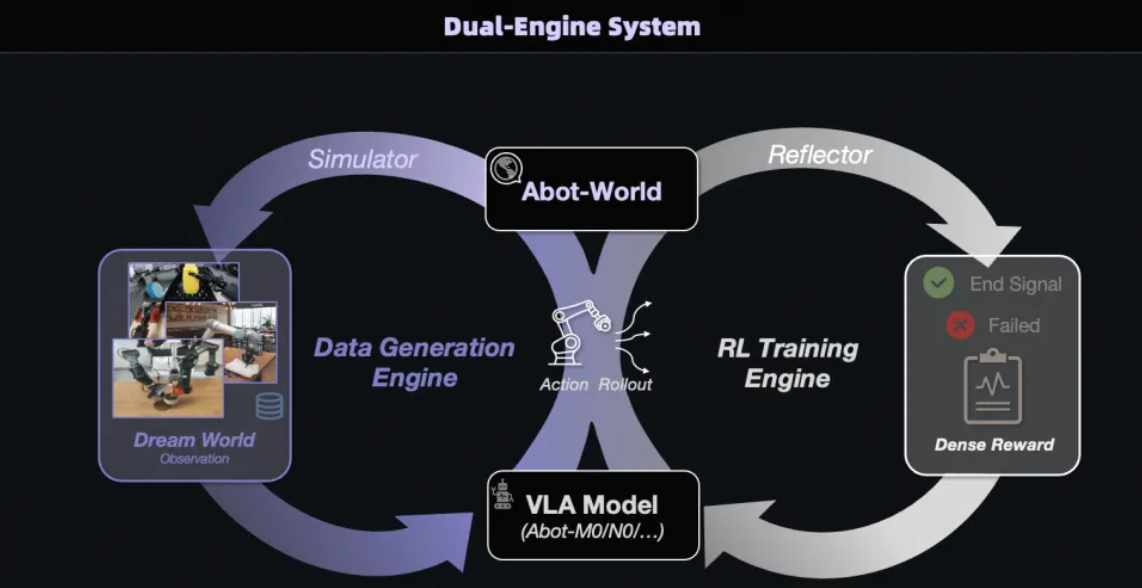
\includegraphics{images/image-0056.png}
\caption{ABot-World 双引擎系统}
\end{figure}

\hypertarget{ux4e8cux4e16ux754cux6a21ux578bux4e0eux7b56ux7565ux6a21ux578bux7684ux95edux73af}{%
\subsubsection{（二）世界模型与策略模型的闭环}\label{ux4e8cux4e16ux754cux6a21ux578bux4e0eux7b56ux7565ux6a21ux578bux7684ux95edux73af}}

ABot-World不是一个静态模型，而是一个具备自我修正能力的认知基座，能接入真实世界的执行反馈，让自己越用越准。VLA和世界模型构成完整的闭环（预测---执行---反馈---自我修正）。例如，机器人根据ABot-World的推演去抓杯子，结果实际执行中夹爪滑脱了。这个误差信号会立刻回传给ABot-PhysWorld，模型自动调整参数，下次预测就会更精准。闭环工作流如下：

\begin{enumerate}
\def\labelenumi{\arabic{enumi}.}
\item
  预测：基于DiT架构，以当前观测和动作为输入，在潜空间中直接生成符合时空动力学的未来状态序列。
\item
  执行：将推演出的最优动作指令下发给机器人执行机构。
\item
  反馈：采集真实世界的执行结果（例如预测能抓起水杯，但实际机械夹爪滑脱了）。
\item
  自我修正：利用真实世界的误差信号反哺认知基座，实时调整模型权重或状态记忆，使得模型``越用越准''。
\end{enumerate}

\hypertarget{ux53c2ux8003ux6587ux732e-205}{%
\subsection{参考文献}\label{ux53c2ux8003ux6587ux732e-205}}

\begin{itemize}
\tightlist
\item
  Wang, R., Liu, Q., Deng, Y., Liu, G., Liu, Z., \& Jia, K. (2026). \href{https://arxiv.org/abs/2603.17808}{EVA: Aligning Video World Models with Executable Robot Actions via Inverse Dynamics Rewards}. arXiv:2603.17808.
\item
  Chen, Y., Chen, R., Huo, D., Yang, Y., Qi, D., Liu, H., Lin, T., Zeng, S., Xiao, J., Chang, X., Xiong, F., Wei, X., Ma, Z., \& Xu, M. (2026). \href{https://arxiv.org/abs/2603.23376}{ABot-PhysWorld: Interactive World Foundation Model for Robotic Manipulation with Physics Alignment}. arXiv:2603.23376.
\end{itemize}

\clearpage

\hypertarget{ux4e16ux754c-ux7b56ux7565ux7edfux4e00ux67b6ux6784ux7684ux5177ux8eabux667aux80fdux8bbaux6587}{%
\section{世界-策略统一架构的具身智能（论文）}\label{ux4e16ux754c-ux7b56ux7565ux7edfux4e00ux67b6ux6784ux7684ux5177ux8eabux667aux80fdux8bbaux6587}}

\begin{quote}
本文是论文阅读笔记，内容代表对对应论文方法或作者理解，不应直接视为领域共识或工程最佳实践。
\end{quote}

\hypertarget{ux4e00ux57faux4e8eux4e16ux754cux6a21ux578bux7684ux5faeux8c03}{%
\subsection{一、基于世界模型的微调}\label{ux4e00ux57faux4e8eux4e16ux754cux6a21ux578bux7684ux5faeux8c03}}

基于具有对物理世界深刻认知的世界模型进行微调，可以获得具身智能需要的``大脑''和训练环境。下面以宇树科技 UnifoLM-WMA-0 为例介绍。

\hypertarget{ux4e00ux5de5ux4f5cux6a21ux5f0f}{%
\subsubsection{（一）工作模式}\label{ux4e00ux5de5ux4f5cux6a21ux5f0f}}

UnifoLM-WMA-0 的核心在于让模型理解机器人与环境相互作用时的物理规律。为了实现这一目标，该架构被设计为支持两种独立但互补的核心工作模式：

\begin{enumerate}
\def\labelenumi{\arabic{enumi}.}
\tightlist
\item
  \textbf{决策模式（Decision-Making Mode / Policy Enhancement）}：执行任务时，世界模型会提前预测机器人在给定动作下与环境物理交互的未来关键信息。这些具有物理常识的``未来特征''，例如物体形变和位移预判，会被输入到动作策略头中，辅助机器人生成更精确的下一步动作。
\item
  \textbf{仿真模式（Simulation Mode / Simulation Engine）}：模型作为交互式物理仿真器运行。输入机器人给定的动作指令后，模型能够自回归地生成高度还原真实场景的物理环境反馈，通常表现为未来视频帧。这相当于在神经网络内部为机器人构建一个可交互的``梦境''环境，可用于生成合成数据以强化学习。
\end{enumerate}

\hypertarget{ux4e8cux6838ux5fc3ux67b6ux6784ux548cux5de5ux4f5cux6d41}{%
\subsubsection{（二）核心架构和工作流}\label{ux4e8cux6838ux5fc3ux67b6ux6784ux548cux5de5ux4f5cux6d41}}

UnifoLM-WMA-0 的训练与部署工作流分为三个阶段，逐步从单纯的``视频生成''过渡到``物理决策''：

\begin{enumerate}
\def\labelenumi{\arabic{enumi}.}
\tightlist
\item
  \textbf{视频生成模型基础微调（World Model Pre-training）}

  \begin{itemize}
  \tightlist
  \item
    输入：海量跨实体机器人数据集（如 Open-X Embodiment Dataset）中的图像观测（Observation）和文本指令（Text Instruction）。
  \item
    处理：对预训练的视频生成扩散模型进行针对性微调，使其生成能力从``生成通用视频''收敛到``生成机器人真实作业场景视频''。
  \item
    输出：具备基础物理直觉的视频大模型。
  \end{itemize}
\item
  \textbf{决策模式后训练（Decision-making Post-training）}

  \begin{itemize}
  \tightlist
  \item
    输入：下游具体任务数据集，例如具体型号机器人的抓取、叠积木动作数据。
  \item
    处理：冻结部分世界模型参数，接入动作头（Action Head）。将世界模型提取的中间特征表征与环境观测共同喂入动作头。
  \item
    输出：优化动作头网络，使其能够输出精确的关节控制指令序列。
  \end{itemize}
\item
  \textbf{仿真模式后训练（Simulation Post-training）}

  \begin{itemize}
  \tightlist
  \item
    输入：当前环境观测、文本指令，以及给定动作序列（Action Condition）。
  \item
    处理：强迫世界模型不仅根据文本预测未来，还严格遵循输入动作序列生成对应的未来物理反馈视频。
  \item
    输出：高保真的交互式神经网络仿真器。
  \end{itemize}
\item
  基于机器人数据、图像和文本指令的基础微调。
\end{enumerate}

\textbf{子步骤 1：独立编码与降维压缩（Encoding \& Compression）}。高分辨率像素图像和离散自然语言文本无法直接在同一个数学空间中计算，因此第一步必须将它们映射到各自的高维连续特征空间中。

\textbf{图像观测处理（Image Observation Processing）}：为了大幅降低扩散模型的计算复杂度，系统通常不会在像素空间直接操作，而是使用预训练变分自编码器（VQ-VAE 或连续 VAE）的编码器模块。设输入的初始图像观测为高分辨率张量 \(o_0 \in \mathbb{R}^{H \times W \times 3}\)，经过编码器后，图像被压缩为隐空间特征图：

\[
z_0 = E(o_0), \qquad z_0 \in \mathbb{R}^{h \times w \times c}
\]

其中 \(h,w\) 是压缩后的空间分辨率，\(c\) 是隐通道数。此时 \(z_0\) 包含当前机器人视角下浓缩的几何与物理状态。

\textbf{文本指令处理（Text Instruction Processing）}：输入的自然语言指令，例如``将红色苹果放入篮子中''，由大语言模型或文本编码器（如 T5 或 CLIP Text Encoder）分词并提取语义特征，转化为上下文嵌入序列：

\[
E_{\mathrm{text}} = T(c_{\mathrm{text}}), \qquad E_{\mathrm{text}} \in \mathbb{R}^{L \times D}
\]

\textbf{子步骤 2：跨模态时空注意力融合（Cross-Modal Attention Fusion）}。扩散模型主干网络通常是 3D U-Net 或 Diffusion Transformer（DiT），它需要把``文本的意思''和``图像的现状''融合进未来画面的生成过程。网络内部主要通过交叉注意力机制实现文本指令对视觉生成的指导。设网络当前层处理的未来视频帧隐变量特征为 \(z_{\mathrm{visual}}\)，则：

\[
Q = W_Q z_{\mathrm{visual}}
\]

\[
K = W_K E_{\mathrm{text}}, \qquad V = W_V E_{\mathrm{text}}
\]

物理解释是：当网络生成``机械臂抓取苹果''的画面时，画面中``机械臂''和``苹果''所在区域的视觉特征会与文本指令中``抓取''和``苹果''的语义向量产生高权重匹配，从而使生成的视频遵循文本约束。

\textbf{子步骤 3：基于条件的隐空间去噪（Conditional Denoising）}。融合图像观测 \(z_0\) 和文本指令 \(E_{\mathrm{text}}\) 后，模型以它们为条件预测未来视频序列噪声。假设预测未来第 \(k\) 帧的隐状态，网络接收加噪的未来隐状态 \(z_t^{(k)}\)，并以拼接或自注意力方式注入初始观测 \(z_0\)。网络相关目标函数可写为：

\[
\mathcal{L}
= \mathbb{E}_{\epsilon \sim \mathcal{N}(0,1), t}
\left[
\left\|
\epsilon - \epsilon_\theta \left(z_t^{(k)}, k, z_0, E_{\mathrm{text}}\right)
\right\|_2^2
\right]
\]

通过优化这一损失，模型学习``看到初始画面 \(z_0\)，并听到指令 \(E_{\mathrm{text}}\) 时，接下来的物理世界应该如何演变''。

\begin{enumerate}
\def\labelenumi{\arabic{enumi}.}
\setcounter{enumi}{1}
\tightlist
\item
  决策模式。
\end{enumerate}

在决策模式下，目标是输出动作 \(a_{\mathrm{pred}}\)。系统会提取世界模型在逆向去噪过程中的中间层特征表示：

\[
f_{\mathrm{WM}}(o_t, c)
\]

这组特征隐含模型对场景几何和动力学规律的高维理解。动作策略头接收该特征，并输出对应动作。对于连续型物理控制任务，采用均方误差（MSE）计算与专家真实动作 \(a_{\mathrm{GT}}\) 的行为克隆损失：

\[
\mathcal{L}_{\mathrm{action}}
= \mathbb{E}_{o_t,c}
\left[
\left\|
a_{\mathrm{GT}} - \pi_\theta(f_{\mathrm{WM}}(o_t,c))
\right\|_2^2
\right]
\]

端到端联合微调时，系统总损失为：

\[
\begin{aligned}
\mathcal{L}_{\mathrm{total}}
&= \lambda_1 \mathcal{L}_{\mathrm{WM}}
\\
&\quad + \lambda_2 \mathcal{L}_{\mathrm{action}}
\end{aligned}
\]

\begin{enumerate}
\def\labelenumi{\arabic{enumi}.}
\setcounter{enumi}{2}
\tightlist
\item
  仿真模式：采用条件扩散模型的损失。
\end{enumerate}

\hypertarget{ux4e8clingbot-vaux57faux4e8e-mot-ux7684ux7b56ux7565ux4e0eux4e16ux754cux6a21ux578bux7edfux4e00}{%
\subsection{二、LingBot-VA：基于 MoT 的策略与世界模型统一}\label{ux4e8clingbot-vaux57faux4e8e-mot-ux7684ux7b56ux7565ux4e0eux4e16ux754cux6a21ux578bux7edfux4e00}}

在具身智能中，世界模型和 VLM/VLA 模型可以合二为一，采用 MoT 架构。下面以 LingBot-VA 为例分析。

\hypertarget{ux4e00ux987aux5e8fux53ccux6d41ux67b6ux6784}{%
\subsubsection{（一）顺序双流架构}\label{ux4e00ux987aux5e8fux53ccux6d41ux67b6ux6784}}

视觉观察首先通过因果视频 VAE 被压缩为紧凑隐变量 \(z_t \in \mathbb{R}^{N \times 4}\)。动作向量也被投影为对应维度的 token。在每个自回归步骤中，模型首先基于观察和动作历史，预测未来 \(K\) 帧视频画面的隐状态：

\[
z_{t+1:t+K} \sim p_\theta(z \mid z_{\le t}, a_{\lt t})
\]

随后，逆动力学模型利用预测的未来视觉状态、历史观察和历史动作，解码出具体动作：

\[
a_{t:t+K-1} \sim q_\phi(a \mid z_{t+1:t+K}, z_{\le t}, a_{\lt t})
\]

需要注意的是，上面的世界模型条件是 \(a_{\lt t}\) 而不是 \(a_{\le t}\)。这是因为第一阶段预测未来画面，第二阶段的逆动力学才根据预测画面推导当前应执行的动作 \(a_t\)。

视频流非常庞大，基于 Wan2.2-5B 预训练模型初始化，隐藏层维度高达 \(d_v=3072\)，因为它需要理解复杂视觉场景和物理动态。动作流则更轻量，深度虽与视频流相同，但隐藏层维度仅为 \(d_a=768\)，约为视频流的四分之一。这是因为动作分布，例如机械臂 7 自由度关节角和 1 维夹爪操作，在本质上比像素级视觉画面简单得多。

在世界模型中，这两个流融合在统一 Transformer 中推理。视频会被降采样，以保证 Transformer 维度对齐。在注意力层，两者统一交互：

\[
\left[z_t', a_{t,1}, a_{t,2}, \ldots, a_{t,r}, z_{t+1}', \ldots\right]
\]

在 MoT 结构中，两种模态通过交叉注意力机制融合特征，同时保持各自特征空间的独立性。

在前馈神经网络或 MoE 层，不同模态分开处理。二者的输出头也是分开的，但对每次输出 token 来说，总是只选择一个。输出时，模型可以在输出序列中交替输出视频 token 和动作 token。

\hypertarget{ux4e8cux5de5ux4f5cux6d41ux4e0eux5f02ux6b65ux63a8ux7406ux65b9ux6cd5}{%
\subsubsection{（二）工作流与异步推理方法}\label{ux4e8cux5de5ux4f5cux6d41ux4e0eux5f02ux6b65ux63a8ux7406ux65b9ux6cd5}}

整体是``块内扩散，块间自回归''，每个块包含 \(r\) 个 token。

\begin{enumerate}
\def\labelenumi{\arabic{enumi}.}
\tightlist
\item
  \textbf{基于 KV-Cache 的同步推理（Algorithm 1）}
\end{enumerate}

这是标准流程，利用大模型的 KV 缓存机制避免历史数据重复计算：

\begin{enumerate}
\def\labelenumi{\arabic{enumi}.}
\item
  获取初始图像 \(o_0\)，通过 VAE 编码为 \(z_0\)，将其存入缓存 \(C_0\)。
\item
  采样随机噪声，结合缓存 \(C\)，通过积分流时间至 \(s=0.5\)，生成未来的视频块预测 \(z_{t+1:t+K}\)。
\item
  基于预测出的视频块和缓存，积分流时间至 \(s=1.0\)，生成未来的动作块 \(a_{t:t+K-1}\)。
\item
  机器人执行动作，收集真实环境的新观察，并将新的 \(z\) 与 \(a\) 追加到缓存 \(C\) 中，循环执行。
\item
  \textbf{FDM-grounded 异步推理（Algorithm 2）}
\end{enumerate}

假设当前系统处于时间步 \(t\)：

\begin{itemize}
\tightlist
\item
  机器人侧：正在花费物理时间执行动作块 \(a_t\)。
\item
  模型侧：必须立刻开始计算下一时间步的动作 \(a_{t+1}\)，以保证 \(a_t\) 执行完后无缝衔接。
\item
  困境：此时现实世界中，执行 \(a_t\) 后的最终真实视觉状态尚未发生，相机无法捕捉。
\end{itemize}

如果采用朴素异步策略，模型会直接从 KV-Cache 里取上一轮在 \(t-1\) 时刻凭空预测出来的幻觉状态，并基于这个过期幻觉继续预测未来的 \(z_{t+1}\)。由于视频生成模型偏好时间平滑性，它会顺着幻觉轨迹一路生成下去，忽视现实世界中已经发生的微小物理偏差，最终导致开环退化和轨迹漂移。

为了打断这种``用幻觉预测幻觉''的恶性循环，系统会提取目前能拿到的最新真实环境反馈，也就是执行 \(a_{t-1}\) 之前的真实观测 \(z_{t-1}\)。

此时模型不使用旧预测，而是执行一次 FDM 前向传播。它将最新真实观测 \(z_{t-1}\) 以及当前电机正在执行的动作 \(a_t\) 一起喂给模型，让模型在真实前置条件下推演``施加该动作后，当前视觉状态应该变成什么样''，得到新的 \(\hat{z}_t\)。

这一步是纠正的核心：系统将这个基于真实数据反馈推演出的 \(\hat{z}_t\) 强制更新进 KV-Cache，替换原本陈旧、未接地的预测。随后，模型基于这个与环境反馈重新对齐的基础，再预测未来的视频块 \(z_{t+1}\) 并解码后续动作序列 \(a_{t+1}\)。

\hypertarget{ux4e09ux4e3aux4ec0ux4e48ux89c6ux89c9ux6d41ux53eaux9700ux8981ux53bbux566aux5230-s0.5ux52a8ux4f5cux6d41ux5fc5ux987bux5230-s1}{%
\subsubsection{\texorpdfstring{（三）为什么视觉流只需要去噪到 \(s=0.5\)，动作流必须到 \(s=1\)？}{（三）为什么视觉流只需要去噪到 s=0.5，动作流必须到 s=1？}}\label{ux4e09ux4e3aux4ec0ux4e48ux89c6ux89c9ux6d41ux53eaux9700ux8981ux53bbux566aux5230-s0.5ux52a8ux4f5cux6d41ux5fc5ux987bux5230-s1}}

简单来说，前者是为了加速，后者是为了精确。

\begin{enumerate}
\def\labelenumi{\arabic{enumi}.}
\tightlist
\item
  \textbf{视觉流}
\end{enumerate}

在自回归生成中，视频画面维度极高，生成视频 token 并进行多步去噪是推理过程最大的延迟来源。作者发现，逆动力学模型并不需要像素级完美的未来画面。只要视频画面能呈现大致的语义结构和运动趋势，动作解码器就能提取足够信息来规划动作。

为让模型具备``看半成品做决策''的能力，训练阶段以 \(p=0.5\) 的概率将历史视觉特征 \(z_{\lt t}\) 替换为部分加噪特征 \(\tilde{z}_{\lt t}\)：

\[
\tilde{z}_{\lt t} = (1-s_{\mathrm{aug}})z_{\lt t} + s_{\mathrm{aug}}\epsilon,
\qquad s_{\mathrm{aug}} \in [0.5, 1]
\]

这里的 \(s_{\mathrm{aug}}\) 模拟未完全去噪状态。通过这种增强，动作解码器被训练出从半模糊视频状态中准确预测动作的鲁棒性。

因此，在实际推理时，视频流不必完全去噪到 \(s=1\)。只需将常微分方程（ODE）积分到 \(s=0.5\)，有些实现中具体到 \(s=0.6\)，即可把半噪声的视频块交给后续动作流使用。这会显著降低视频生成的去噪步数和计算开销。

\begin{enumerate}
\def\labelenumi{\arabic{enumi}.}
\setcounter{enumi}{1}
\tightlist
\item
  \textbf{动作流}
\end{enumerate}

半模糊视频可以看懂，但半噪声动作无法在物理世界中执行。机器人的动作空间包含末端位姿、旋转四元数、关节角度和夹爪开合等连续数值，任何残余噪声都可能造成碰撞或抓取失败。因此动作流必须完整积分到 \(s=1.0\)，获得干净、确定的动作指令。

得益于非对称 MoT 架构，动作流隐藏层维度较低，仅为视频流宽度的四分之一，参数量也小。对低维动作数据进行完整 ODE 积分的额外计算开销很小，不会像视频生成那样成为系统瓶颈。

\hypertarget{ux4e09ux7269ux7406-token-ux7684ux7edfux4e00ux81eaux56deux5f52ux9884ux6d4b}{%
\subsection{三、物理 token 的统一自回归预测}\label{ux4e09ux7269ux7406-token-ux7684ux7edfux4e00ux81eaux56deux5f52ux9884ux6d4b}}

PAR、PhysGen 等论文以及 NVIDIA DreamDojo 提出了把状态与策略统一编码到``物理 token''中，统一自回归生成，再在下游解码为状态与策略输出的范式。

\hypertarget{ux4e00ux6838ux5fc3ux601dux60f3-28}{%
\subsubsection{（一）核心思想}\label{ux4e00ux6838ux5fc3ux601dux60f3-28}}

将过去的视频和动作编码为统一物理 token。设 \(t\) 时刻的视频帧 token 集合为 \(o_t\)，动作 token 集合为 \(a_t\)，则上下文序列为：

\[
\left[\mathrm{prompt}, o_1, a_1, o_2, a_2, \ldots, o_t, a_t\right]
\]

模型联合预测下一步的 \([o_{t+1}, a_{t+1}]\)。预测出的 \([o_{t+1}, a_{t+1}]\) 再通过扩散解码，分别得到连续的未来状态值（视频）和要采取的动作值。

具体而言，\(o_t\) 和 \(a_t\) 的生成方式并不相同：\(o_t\) 内部 token 可以并行生成，\(a_t\) 内部则按时间顺序严格串行。借助 multi-token prediction，模型在动作块内部拉长微观规划视野，即使需要预判 2 到 5 步极小的机械臂位姿变化，也能让自回归生成的动作轨迹更连贯，避免控制上的短视和抖动。

\begin{figure}[htbp]
\centering
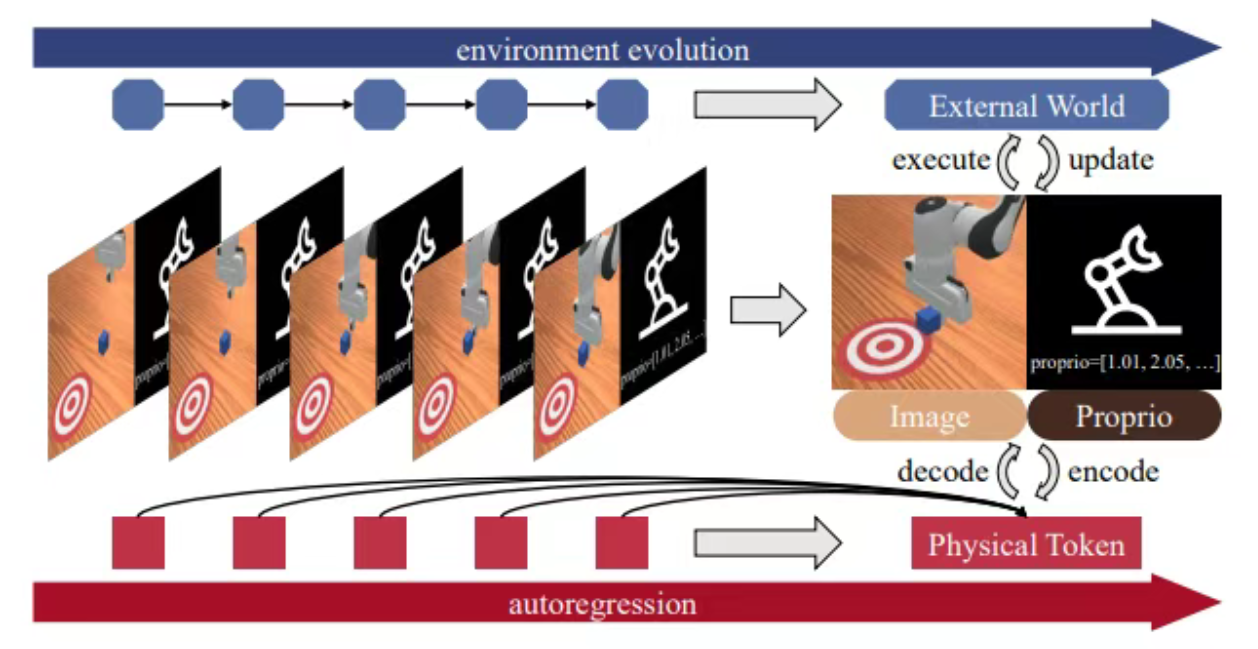
\includegraphics{images/image-0057.png}
\caption{PhysGen 物理 token 自回归示意图}
\end{figure}

\hypertarget{ux4e8cux81eaux56deux5f52-transformer}{%
\subsubsection{（二）自回归 Transformer}\label{ux4e8cux81eaux56deux5f52-transformer}}

主干 Transformer 网络采用自回归生成范式，因果掩码方式如下。

\begin{enumerate}
\def\labelenumi{\arabic{enumi}.}
\tightlist
\item
  \textbf{帧内部：块级全注意力}
\end{enumerate}

对于物理 token 中的视频帧部分，掩码允许同一画面内的所有图像块相互可见。单帧图像内部的空间信息是同时存在的，没有时间先后顺序。全注意力机制可以保证模型完整提取该帧全局空间特征。

\begin{enumerate}
\def\labelenumi{\arabic{enumi}.}
\setcounter{enumi}{1}
\tightlist
\item
  \textbf{动作内部：时间因果注意力}
\end{enumerate}

对于物理标记中的动作部分，模型执行严格的时间因果掩码。一个时间步的动作块内部，各个 token 仍有先后顺序，靠前动作标记不能关注排在后面的动作标记。这对应``过去决定未来，未来不能干涉过去''的物理约束。

\begin{enumerate}
\def\labelenumi{\arabic{enumi}.}
\setcounter{enumi}{2}
\tightlist
\item
  \textbf{动作单向关注视觉}
\end{enumerate}

在同一个时间步 \(t\) 中，动作 token 被允许单向关注视频 token。这使模型学习``给定目标状态，反推动作''的逆运动学推导。

\begin{enumerate}
\def\labelenumi{\arabic{enumi}.}
\setcounter{enumi}{3}
\tightlist
\item
  \textbf{跨时间步：全局时间因果}
\end{enumerate}

不同时间步之间严格遵守时间因果掩码，用 \(t\) 时刻以前的信息预测 \(t+1\) 时刻，防止未来帧信息泄露到过去规划中。

\hypertarget{ux4e09ux6269ux6563ux89e3ux7801ux5668}{%
\subsubsection{（三）扩散解码器}\label{ux4e09ux6269ux6563ux89e3ux7801ux5668}}

与传统离散分类不同，PhysGen 引入基于 DiT（Diffusion Transformer）的去噪过程，利用扩散损失直接在连续空间中估计概率分布。模型被训练来预测注入噪声，从而最小化均方误差损失：

\[
\begin{aligned}
\mathcal{L}(P_n, z_n)
&= \mathbb{E}_{\epsilon,t}
\left[
\left\|
\epsilon - \epsilon_\theta(P_{n,t}\mid t,z_n)
\right\|_2^2
\right]
\end{aligned}
\]

推理阶段去噪公式为：

\[
\begin{aligned}
P_{n,t-1}
&=
\frac{1}{\sqrt{\alpha_t}}
\left(
P_{n,t}
\, - \, \frac{1-\alpha_t}{\sqrt{1-\bar{\alpha}_t}}
\epsilon_\theta(P_{n,t}\mid t,z_n)
\right)
\\
&\quad + \sigma_t \epsilon
\end{aligned}
\]

去噪后的物理标记最终被分离，并解码为预测视频帧和真实世界中要执行的机器人动作。

\hypertarget{ux56dbboa-token}{%
\subsubsection{（四）BOA token}\label{ux56dbboa-token}}

真实物理世界中的因果关系非常严格。假设一个机器人需要完成任务：

\begin{itemize}
\tightlist
\item
  初始时刻 \(t=0\)：机器人看到桌子上的杯子，获得初始视觉观察结果 Frame 0，但此时还没有执行任何动作。
\item
  第一步 \(t=1\)：机器人处理 Frame 0 的信息，决定伸出机械臂并输出第一个动作 Action 1。因为这个动作，物理世界发生变化，机器人看到新的画面 Frame 1。
\end{itemize}

PhysGen 的特色是把帧标记（Frame token）和动作标记（Action token）拼在一起，组成统一的物理标记 \(P_n\) 来进行自回归预测：

\[
P_n = [F_{o,n}; F_{a,n}]
\]

按照物理直觉，输入模型的历史序列是：

\begin{itemize}
\tightlist
\item
  视觉观察序列：\(\{O_0,O_1,O_2,\ldots,O_{N-1}\}\)，从 0 开始，多一个初始帧。
\item
  对应动作序列：\(\{A_1,A_2,\ldots,A_{N-1}\}\)，从 1 开始，少一个初始动作。
\end{itemize}

如果强行两两打包，就会遇到时间偏移问题：

\begin{itemize}
\tightlist
\item
  \(P_0 = [O_0; \varnothing]\)，这里对不齐。
\item
  \(P_1 = [O_1; A_1]\)
\item
  \(P_2 = [O_2; A_2]\)
\end{itemize}

为在数学结构上对齐这两个长度不同的序列，让它们能放入 Transformer，作者在动作序列最前面人为塞入一个可学习占位符，称为 BOA（Begin of Action）token。

\hypertarget{ux4e94ux8badux7ec3ux5de5ux4f5cux6d41}{%
\subsubsection{（五）训练工作流}\label{ux4e94ux8badux7ec3ux5de5ux4f5cux6d41}}

\begin{enumerate}
\def\labelenumi{\arabic{enumi}.}
\tightlist
\item
  \textbf{预训练}
\end{enumerate}

预训练阶段，模型主干网络只在海量视频数据上训练。此时模型尚未见过机器人动作指令，学习的是``世界如何运转''，例如杯子掉到地上会碎、手碰到物体会让物体移动等物理和时间动态。

该阶段只训练语言 tokenizer、视觉 tokenizer（如 D-VAE）、自回归 Transformer 主干以及帧生成器（Frame Diffusion），动作模块不参与。

\begin{enumerate}
\def\labelenumi{\arabic{enumi}.}
\setcounter{enumi}{1}
\tightlist
\item
  \textbf{动作微调}
\end{enumerate}

为了让模型控制机器人，作者会在具体下游任务上进行微调（Fine-tuning）。这一阶段使用带动作标签的演示数据。因为模型在第一阶段已经学习到物理世界运作规律，所需动作数据量可以较小。

此时模型会增加用于编码动作的 Action Tokenizer（一个 MLP）以及轻量级动作解码器（Action-DiT）。微调时，模型被训练为：一旦看到 BOA token，后续就按``60 个视频帧 token + 8 个动作 token''的模式交替生成，系统再按 token 类型分发给不同解码器。

\hypertarget{ux53c2ux8003ux6587ux732e-206}{%
\subsection{参考文献}\label{ux53c2ux8003ux6587ux732e-206}}

\begin{itemize}
\tightlist
\item
  Unitree Robotics. (2025). \href{https://github.com/unitreerobotics/unifolm-world-model-action}{UnifoLM-WMA-0: World-Model-Action Architecture for General Robots}. GitHub repository.
\item
  Li, L., Zhang, Q., Yu, M., Gao, Z., Luo, Y., Xue, N., Yang, S., Zhu, X., Wang, R., Shen, Y., Han, F., \& Xu, Y. (2026). \href{https://arxiv.org/abs/2601.21998}{Causal World Modeling for Robot Control}. arXiv:2601.21998.
\end{itemize}

\clearpage

\hypertarget{ux4ec5ux5728ux8badux7ec3ux65f6ux878dux5165ux9884ux6d4bux80fdux529bux7684ux5177ux8eabux667aux80fdux8bbaux6587}{%
\section{仅在训练时融入预测能力的具身智能（论文）}\label{ux4ec5ux5728ux8badux7ec3ux65f6ux878dux5165ux9884ux6d4bux80fdux529bux7684ux5177ux8eabux667aux80fdux8bbaux6587}}

\begin{quote}
本文是论文阅读笔记，内容代表对对应论文方法或作者理解，不应直接视为领域共识或工程最佳实践。
\end{quote}

\hypertarget{ux4e00fast-wamux4ec5ux5728ux8badux7ec3ux65f6ux9884ux6d4bux72b6ux6001ux7684ux63a8ux7406}{%
\subsection{一、Fast-WAM：仅在训练时预测状态的推理}\label{ux4e00fast-wamux4ec5ux5728ux8badux7ec3ux65f6ux9884ux6d4bux72b6ux6001ux7684ux63a8ux7406}}

\hypertarget{ux4e00ux95eeux9898ux80ccux666f-22}{%
\subsubsection{（一）问题背景}\label{ux4e00ux95eeux9898ux80ccux666f-22}}

在具身智能领域，视觉-语言-动作模型（VLA, Vision-Language-Action），例如 OpenVLA、RT-2 等，在过去取得了巨大进展。然而，传统 VLA 主要基于静态图文数据进行预训练，缺乏对物理世界动态演变过程的建模。

为了解决这一问题，AI 领域发展出一条新的技术路线：世界动作模型（WAMs, World Action Models）。WAMs 将``预测未来视觉画面''与``预测机器人动作''结合在统一框架中，使模型具备物理先验知识。

现有 WAMs 大多遵循``先想象，后执行''（imagine-then-execute）的范式：推理时，模型必须先生成未来视频帧，再基于这些预测未来画面输出动作。该范式的致命弱点是推理延迟高。测试时需要通过扩散模型迭代去噪生成视频，使模型很难在机器人上实现低延迟实时控制。

因此，Fast-WAM 提出核心问题：WAMs 是否真的需要在测试时显式``想象''未来画面？还是说，性能提升主要来自训练阶段的视频预测协同训练（Video Co-training），它让模型学到了更好的物理世界表征？

\hypertarget{ux4e8cux57faux5ea7ux6a21ux578b}{%
\subsubsection{（二）基座模型}\label{ux4e8cux57faux5ea7ux6a21ux578b}}

Fast-WAM 采用开源视频扩散 Transformer Wan2.2-5B 作为世界建模骨干网络，复用 Wan2.2 的视频 DiT、文本编码器 T5 以及视频 VAE。

\hypertarget{ux4e09ux6a21ux578bux67b6ux6784ux4e0eux8badux7ec3ux5de5ux4f5cux6d41}{%
\subsubsection{（三）模型架构与训练工作流}\label{ux4e09ux6a21ux578bux67b6ux6784ux4e0eux8badux7ec3ux5de5ux4f5cux6d41}}

\textbf{第一步：Token 的精确分组}。在送入 MoT 架构前，所有输入信息被严格划分为三个 token 组：

\begin{enumerate}
\def\labelenumi{\arabic{enumi}.}
\tightlist
\item
  视觉锚点 \(f_0\)：当前第一帧观测图像的干净潜在特征，不加噪。
\item
  未来视频 \(f_{1:h}\)：未来视频帧的加噪潜在特征，仅在训练时存在。
\item
  动作序列 \(a_{1:h}\)：要生成的动作块的加噪特征。
\end{enumerate}

这里的``第一帧''是相对于原本要生成的未来视频块而言的锚点（Anchor）。模型摒弃了推理时生成未来画面的过程，而是将唯一一帧当前图像输入视频骨干网络做一次单向前向传播，提取世界表征，然后直接交给动作专家网络生成后续动作序列。这种设计使 Fast-WAM 具备类似标准 VLA 的快速实时响应能力。

\textbf{第二步：全局文本 Cross-Attention 注入}。在这三个 token 组进入 DiT 每一层时，所有 token 组都会通过 Cross-Attention 关注语言特征向量。数学上，\(f_0\)、\(f_{1:h}\) 和 \(a_{1:h}\) 都作为 Query，文本特征作为 Key 和 Value。其物理意义是：无论提取当前视觉特征、推演未来物理变化，还是规划具体动作，都始终受到人类语言指令引导。

\textbf{第三步：结构化 Self-Attention 掩码}。注入文本信息后，token 之间需要在 DiT 内部进行自注意力交互。作者设计严格注意力掩码来控制信息流：

\begin{itemize}
\tightlist
\item
  Video DiT 内部交互：未来加噪视频 token \(f_{1:h}\) 可以在视频分支内双向互相关注，并允许关注第一帧干净特征 \(f_0\)，使模型基于初始状态推演未来。
\item
  Action DiT 内部交互：动作 token \(a_{1:h}\) 可以在动作分支内双向互相关注，同样允许关注第一帧干净特征 \(f_0\)，使模型基于当前视觉状态规划连贯动作序列。
\item
  不可跨越的红线：动作 token 绝对不允许关注未来视频 token；同时，第一帧干净 token \(f_0\) 不关注任何其他 token，避免被噪声污染。
\end{itemize}

严禁越界的原因是：如果训练时动作特征能看到未来视频特征，动作专家会产生依赖，根据``未来已经发生的结果''反推``现在该做什么动作''。但在真实部署时，为追求约 190 毫秒的低延迟，Fast-WAM 会直接移除未来视频生成分支。若模型训练时依赖未来视频，推理时就会因输入缺失而崩溃。因此，结构化掩码强迫动作预测只能立足当前帧和文本，从根本上解耦训练时视频辅助和推理时动作生成。

\hypertarget{ux56dbux635fux5931ux51fdux6570-3}{%
\subsubsection{（四）损失函数}\label{ux56dbux635fux5931ux51fdux6570-3}}

对于目标变量 \(y\)，它既可以是动作序列 \(a_{1:h}\)，也可以是未来视频特征 \(z_{1:T}\)。算法采样高斯噪声 \(\epsilon \sim \mathcal{N}(0,I)\) 和时间步 \(t \in (0,1)\)，构建插值样本：

\[
y_t = (1-t)y + t\epsilon
\]

模型通过标准流匹配损失预测速度场：

\[
\begin{aligned}
\mathcal{L}_{\mathrm{FM}}(y)
&= \mathbb{E}_{y,\epsilon,t}
\left[
\left\|
f_\theta(y_t,t,o,l) - (\epsilon-y)
\right\|_2^2
\right]
\end{aligned}
\]

总优化目标是动作损失和视频协同训练损失的加权和：

\[
\begin{aligned}
\mathcal{L}
&= \mathcal{L}_{\mathrm{act}}
\\
&\quad + \lambda \mathcal{L}_{\mathrm{vid}}
\end{aligned}
\]

\hypertarget{ux4e94ux63a8ux7406ux5de5ux4f5cux6d41-1}{%
\subsubsection{（五）推理工作流}\label{ux4e94ux63a8ux7406ux5de5ux4f5cux6d41-1}}

推理阶段彻底抛弃显式视频生成，实现极快响应：

\begin{enumerate}
\def\labelenumi{\arabic{enumi}.}
\tightlist
\item
  \textbf{单次前向传递}：仅保留第一帧干净潜在特征，将其输入视频骨干网络进行一次单向前向传播，提取具有物理意义的潜在世界表征 \(z(o,l)\)。
\item
  \textbf{直接动作去噪}：动作专家 DiT 直接基于该表征参数化动作分布：
\end{enumerate}

\[
p_\theta(a_{1:H}\mid z(o,l))
\]

\begin{enumerate}
\def\labelenumi{\arabic{enumi}.}
\setcounter{enumi}{2}
\tightlist
\item
  \textbf{输出执行}：由于不需要对未来视频帧实例化和去噪，动作生成仅需少量无分类器引导（CFG=1.0）的去噪步即可输出动作序列。
\end{enumerate}

\hypertarget{ux516dux5b9eux9a8cux7ed3ux679c}{%
\subsubsection{（六）实验结果}\label{ux516dux5b9eux9a8cux7ed3ux679c}}

\begin{enumerate}
\def\labelenumi{\arabic{enumi}.}
\tightlist
\item
  \textbf{极低推理延迟}：真实机器人任务中，Fast-WAM 延迟约 190 毫秒，而采用``先想象后执行''的 Fast-WAM-IDM 延迟高达约 810 毫秒，Fast-WAM 实现超过 4 倍提速。
\item
  \textbf{性能接近前沿方法}：在没有进行大规模具身预训练（Embodied Pretraining）的情况下，Fast-WAM 在 RoboTwin 上取得 91.8\% 的成功率，在 LIBERO 上取得 97.6\% 的平均成功率，不仅优于不带视频预测的 VLA 基线，也接近最强预训练 WAMs。
\item
  \textbf{回答核心假设}：Fast-WAM 的表现与显式生成未来的变体（Joint 和 IDM）非常接近。但如果移除训练时的视频协同训练任务（w.o. video co-train），RoboTwin 成功率下降到 83.8\%，真机折叠毛巾任务成功率也显著下降。
\end{enumerate}

最终结论：WAMs 强大的根本原因在于训练阶段的视频预测任务重塑了模型的物理世界表征能力，而不在于推理阶段显式生成未来画面。Fast-WAM 说明，可以在训练时利用世界模型带来的物理先验，在部署时仍保持 VLA 式的快速响应。

\hypertarget{ux4e8cbeing-h0.7ux8badux7ec3ux65f6ux8ba9ux52a8ux4f5cux9884ux6d4bux4e0eux57faux4e8eux672aux6765ux72b6ux6001ux7684ux52a8ux4f5cux9884ux6d4bux5bf9ux9f50}{%
\subsection{二、Being-H0.7：训练时让``动作预测''与``基于未来状态的动作预测''对齐}\label{ux4e8cbeing-h0.7ux8badux7ec3ux65f6ux8ba9ux52a8ux4f5cux9884ux6d4bux4e0eux57faux4e8eux672aux6765ux72b6ux6001ux7684ux52a8ux4f5cux9884ux6d4bux5bf9ux9f50}}

\hypertarget{ux4e00ux95eeux9898ux80ccux666f-23}{%
\subsubsection{（一）问题背景}\label{ux4e00ux95eeux9898ux80ccux666f-23}}

具身大模型主要有两条技术路线，但均存在明显局限：

\begin{enumerate}
\def\labelenumi{\arabic{enumi}.}
\tightlist
\item
  \textbf{VLA（视觉-语言-动作模型）}：这类模型如 RT-2、OpenVLA 等，将当前视觉和语言观察直接映射为底层控制动作。痛点是机器人动作数据稀疏且缺乏多样性，模型容易出现行为崩溃（behavior collapse），依赖表面统计相关性，而未学到基于物理规律、具有组合泛化能力的动作表征。
\item
  \textbf{WAM（世界-动作模型）}：基于视频生成模型构建，通过预测未来像素帧演变推断世界动态。痛点包括推理阶段实时生成未来视频帧带来极高计算延迟、像素预测瑕疵会传递到动作解码并导致长周期任务失败，以及训练成本较高。
\end{enumerate}

\hypertarget{ux4e8cux6838ux5fc3ux601dux60f3-8}{%
\subsubsection{（二）核心思想}\label{ux4e8cux6838ux5fc3ux601dux60f3-8}}

Being-H0.7 不需要在像素层面预测未来，而是在训练时让动作预测与基于未来状态的动作预测对齐。模型引入一组可学习的 Latent Queries，在 Transformer 前向传播中不断从多模态上下文中萃取任务相关信息，将其压缩重组并生成动作。训练时，模型还将观测到的未来状态压缩到 latent 空间，同样从多模态上下文中萃取任务相关信息并生成动作；然后让前者（先验分支）向后者（后验分支）对齐。

为了让推理空间真正具备``预测未来''的世界建模能力，作者设计训练期双分支联合对齐（Dual-Branch Joint Alignment）架构：

\begin{itemize}
\tightlist
\item
  \textbf{Prior Branch（先验分支）}：最终用于实机部署的干线分支，仅依赖当前指令和观察，使用 Latent Queries 生成动作。
\item
  \textbf{Posterior Branch（后验分支）}：仅存在于训练阶段的辅助分支，将干线中的 Latent Queries 替换为通过视觉编码器提取的未来观察嵌入（Future Embeddings）。
\item
  \textbf{对齐机制}：在隐藏层特征级别计算先验分支与后验分支的对齐损失，迫使先验分支在只看到当下画面时，推断出与``看到未来''相同的特征表示。
\end{itemize}

\hypertarget{ux4e09ux8badux7ec3ux5de5ux4f5cux6d41-4}{%
\subsubsection{（三）训练工作流}\label{ux4e09ux8badux7ec3ux5de5ux4f5cux6d41-4}}

\textbf{步骤 1：上下文编码与序列构建}。给定任务指令 \(x\)、时间长度为 \(H\) 的历史观测 \(O_{-H:0}\) 以及机器人本体状态 \(s\)。将这些特征映射并拼接后，算法在动作块 \(a_{0:T}\) 的预测序列前插入数量为 \(K\)、维度为 \(d\) 的潜在查询矩阵 \(Q \in \mathbb{R}^{K \times d}\)，构建先验分支的完整 Transformer 序列：

\[
S = \left[x; O_{-H:0}; s; Q; a_{0:T}\right]
\]

\textbf{步骤 2：后验分支的未来特征提取}。算法同步获取未来真实观测视频帧 \(O_{0:T}\)。使用冻结的预训练 ViT 和 Perceiver 重采样器 \(E\)，将其压缩成大小与 \(Q\) 一致的未来嵌入：

\[
z^{\mathrm{post}} = E(O_{0:T}) \in \mathbb{R}^{K \times d}
\]

\textbf{步骤 3：混合 Transformer（MoT）双分支前向传播}。为提高计算效率，算法不串行执行两次大型前向传播，而是利用 Mixture-of-Transformers 架构将两个分支打包成一个长序列。在这个过程中应用双分支注意力掩码（Dual-Branch Attention Mask）：保证两个分支都能看到共享上下文 \(c=[x;O_{-H:0};s]\)，但先验分支和后验分支的 tokens 彼此不可见。

\textbf{步骤 4：损失函数计算}。整个框架通过三个损失函数进行联合优化。

\begin{enumerate}
\def\labelenumi{\arabic{enumi}.}
\tightlist
\item
  \textbf{动作流匹配损失（Flow Matching Loss）}：基于扩散生成范式，为两个分支分别计算对加噪动作的去噪速度场损失。若真实动作为 \(a\)、加噪时间为 \(t\)、目标速度为 \(u_t=a-\epsilon\)，则：
\end{enumerate}

\[
\begin{aligned}
\mathcal{L}_{\mathrm{FM}}^{\mathrm{prior}}
&=
\left\|
v_\theta^{\mathrm{prior}}(a_t,c) - u_t
\right\|_2^2
\end{aligned}
\]

\[
\begin{aligned}
\mathcal{L}_{\mathrm{FM}}^{\mathrm{post}}
&=
\left\|
v_\theta^{\mathrm{post}}(a_t,c,z^{\mathrm{post}}) - u_t
\right\|_2^2
\end{aligned}
\]

\begin{enumerate}
\def\labelenumi{\arabic{enumi}.}
\setcounter{enumi}{1}
\tightlist
\item
  \textbf{隐状态联合对齐损失（Joint Alignment Loss）}：在第 \(l\) 个包含对齐的 Transformer 层，提取先验分支隐状态 \(h_l^{\mathrm{prior}}\) 与后验分支隐状态 \(h_l^{\mathrm{post}}\)，计算均方误差，促使先验空间涌现对未来的世界建模能力：
\end{enumerate}

\[
\begin{aligned}
\mathcal{L}_{\mathrm{align}}
&=
\frac{1}{L}
\sum_{l=1}^{L}
\left\|
h_l^{\mathrm{prior}} - h_l^{\mathrm{post}}
\right\|_2^2
\end{aligned}
\]

\begin{enumerate}
\def\labelenumi{\arabic{enumi}.}
\setcounter{enumi}{2}
\tightlist
\item
  \textbf{防崩溃正则化损失（Regularization Loss）}：为防止对齐导致隐特征趋于全 0 或方向单一化，施加范数和秩的惩罚。范数正则化防止幅值收缩：
\end{enumerate}

\[
\begin{aligned}
\mathcal{R}_{\mathrm{norm}}(h)
&=
\left[
\mathrm{ReLU}(\tau - \lVert h\rVert_2)
\right]^2
\end{aligned}
\]

秩正则化防止方向坍缩，由 Gram 矩阵 \(G\) 的归一化特征值 \(p_i\) 的信息熵表示：

\[
\begin{aligned}
\mathcal{R}_{\mathrm{rank}}(H)
&=
\sum_{i=1}^{B} p_i \log p_i
\end{aligned}
\]

\hypertarget{ux56dbux63a8ux7406ux5de5ux4f5cux6d41-1}{%
\subsubsection{（四）推理工作流}\label{ux56dbux63a8ux7406ux5de5ux4f5cux6d41-1}}

由于模型解耦了特征对齐和前向生成，推理阶段非常轻量：

\begin{enumerate}
\def\labelenumi{\arabic{enumi}.}
\tightlist
\item
  \textbf{观察采集}：机器人摄像头实时采集当前画面，处理并拼接为上下文向量。
\item
  \textbf{纯先验分支执行}：完全丢弃训练时的后验分支和所有未来视频输入，只保留 Transformer 骨干、Latent Queries \(Q\) 以及用于扩散的 Flow Matching 生成头。
\item
  \textbf{动作块输出与 UAC 异步控制}：模型一次性快速生成连续未来动作块 \(a_{0:T}\)。真实部署中结合通用异步分块机制（UAC）：服务器端异步推理未来动作序列，机器人驱动端从线程安全缓冲池中持续取出历史前缀锁定动作执行，两者解耦，以约 \(3\) 到 \(4\) ms/step 的低延迟实现平滑动态控制。
\end{enumerate}

\hypertarget{ux53c2ux8003ux6587ux732e-207}{%
\subsection{参考文献}\label{ux53c2ux8003ux6587ux732e-207}}

\begin{itemize}
\tightlist
\item
  Yuan, T., Dong, Z., Liu, Y., \& Zhao, H. (2026). \href{https://arxiv.org/abs/2603.16666}{Fast-WAM: Do World Action Models Need Test-time Future Imagination?}. arXiv:2603.16666.
\end{itemize}

\clearpage
